One of the main components of the analysis is the 2D fit to the data in the signal region, 
as it extracts the signal yield and significance.
The accuracy on the signal extraction depends on the ability of the fit in determining 
and constraining the backgrounds.
In fact, we first estimate the contribution from the various background processes 
either from data control regions or from MC (see Sec.~\ref{sec:backgrounds}), 
but then we rely on the fit to determine the final yield values. 

We validate the fit performance in presence of a 125 \GeV\ SM Higgs using toy experiments 
under different initial conditions.
Goal of the study is to determine the fit resolution and to check that it does not lead to 
biases in the signal strenght measurement. The procedure is defined as follows.

\begin{itemize}
\item Several thousands toy experiments are thrown with a simple poissonian sampling of S+B central shape (statistical only sampling)
or including systematic variations, both in normalization and shape (statistical+systematic sampling). 
\item Toy experiments can be thrown from nominal or biassed inputs; biases can be due either to normalization or to shape. 
In case of nominal input, toys are sampled from the sum of central shapes normalized to the process yield used in the cards;
in case of normalization bias, one of the yields is varied with respect to the value in the cards; 
in case of shape bias, one of the alternative shapes is used in place of the central when sampling the toys.
\item For each toy a new data card is created, where the data yield and shape are obtained from the sampling.
In case of nominal analysis, all other components in the cards are unchanged; 
in some cases, one systematic value can be inflated to test the ability of the fit in determining 
the nuisance parameter without constraints.
\item Data cards are processed as in the real data analysis; in particular we look at post-fit normalizations 
and at the signal strenght for the signal+background fit.
\end{itemize}

We first test the fit performance without any input bias. 
Figure~\ref{fig:toyfit_statonly_0j}-\ref{fig:toyfit_statonly_1j} show the distributions of the relative fit biases 
for the signal and key background processes in the 0 and 1 Jet bins respectively. 
The signal is estimated without large bias ($\leq 4$\%) and the resolution is 28\% (35\%) in the 0-jet (1-jet) bin 
when toy are sampled with statistical variations only. 
On average we do not find biases on the main background processes either. 
We have also tested the fit performance including systematic effects, where the 
toy datasets are generated sampling over all the systematic nuisance parameters except the normalization 
uncertainties on the $WW$ as it is floated freely in the fit. 
Figure~\ref{fig:toyfit_0j}-\ref{fig:toyfit_1j} show the distributions of the relative fit biases 
for the signal and key background processes in the 0 and 1 Jet bins respectively in this configuration.  
We find that including the systematic effects does not introduce additional bias on both 
signal and background yields. But it worsens the signal resolution by $\sim$30-40\% as expected.  


%%%%%%%%%%%%%%%%%%%%%%%%%%%%%%%%%%%%
\begin{figure}[!hbtp]
\centering
\subfigure[ggH]{
\centering
\label{subfig:ggh}
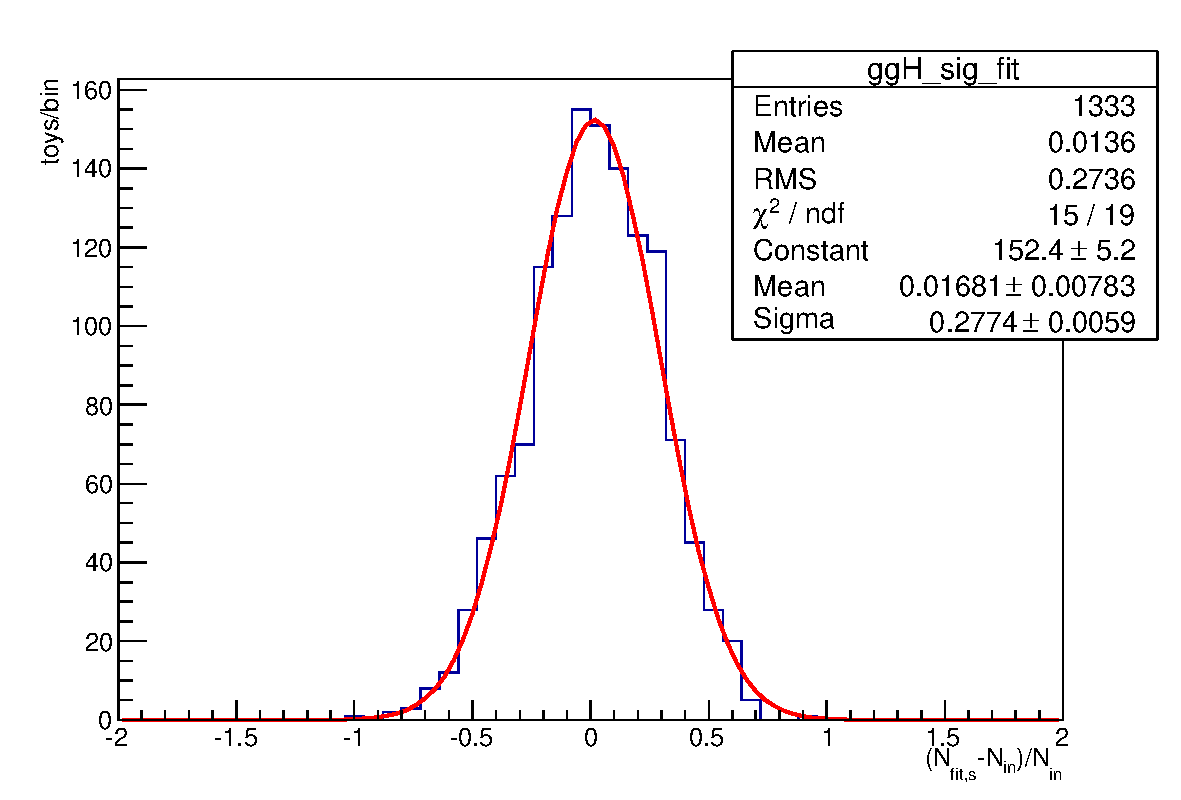
\includegraphics[width=.45\textwidth]{figures/norm_inj125_0j_125_sfit_ggH_hww_statonly.pdf}
}
\subfigure[qqWW]{
\centering
\label{subfig:qqww}
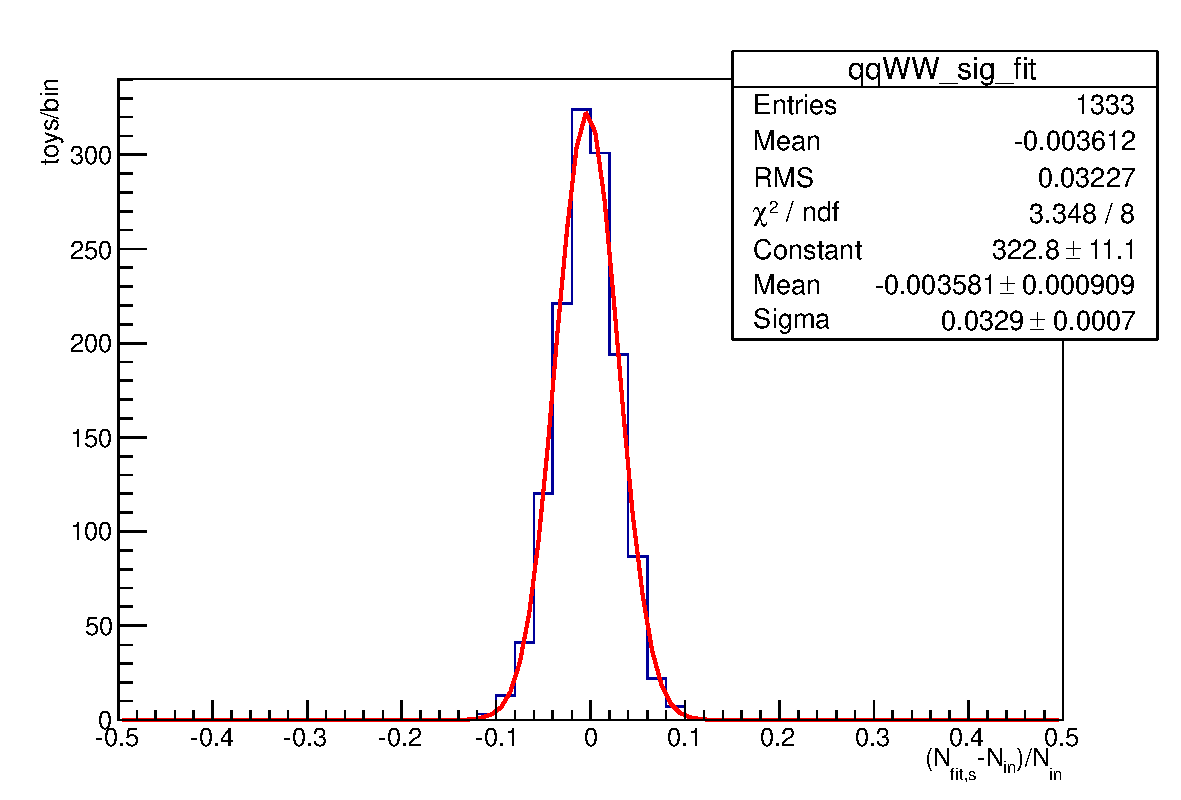
\includegraphics[width=.45\textwidth]{figures/norm_inj125_0j_125_sfit_qqWW_hww_statonly.pdf}
}\\
\subfigure[ggWW]{
\centering
\label{subfig:ggww}
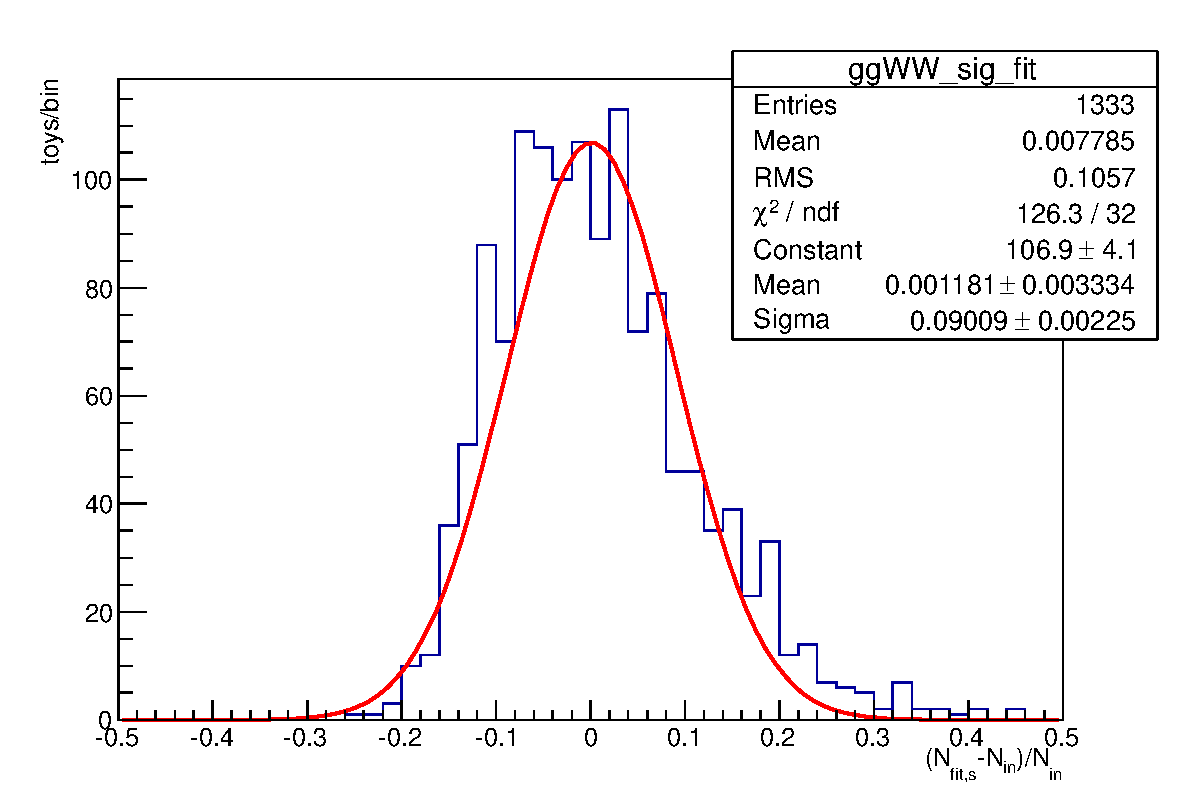
\includegraphics[width=.45\textwidth]{figures/norm_inj125_0j_125_sfit_ggWW_hww_statonly.pdf}
} 
\subfigure[Top]{
\centering
\label{subfig:top}
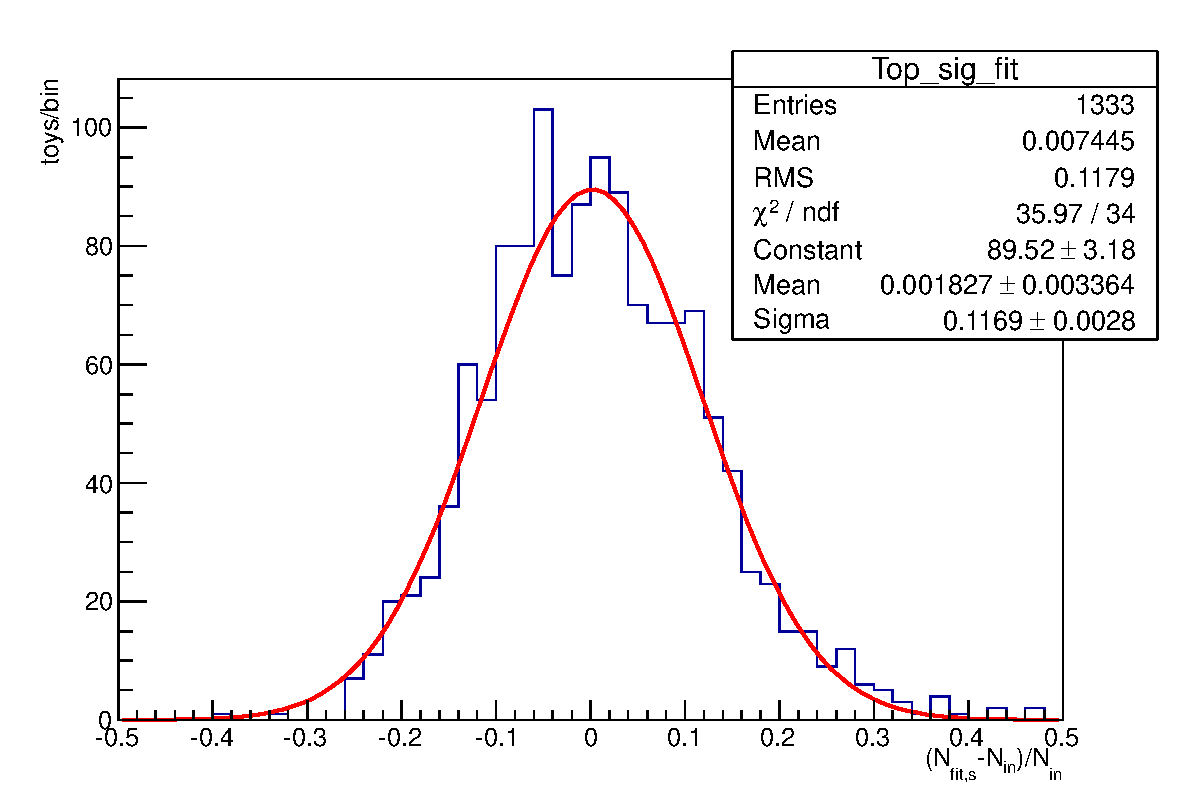
\includegraphics[width=.45\textwidth]{figures/norm_inj125_0j_125_sfit_Top_hww_statonly.pdf}
} \\
\subfigure[WjetsE]{
\centering
\label{subfig:wjetse}
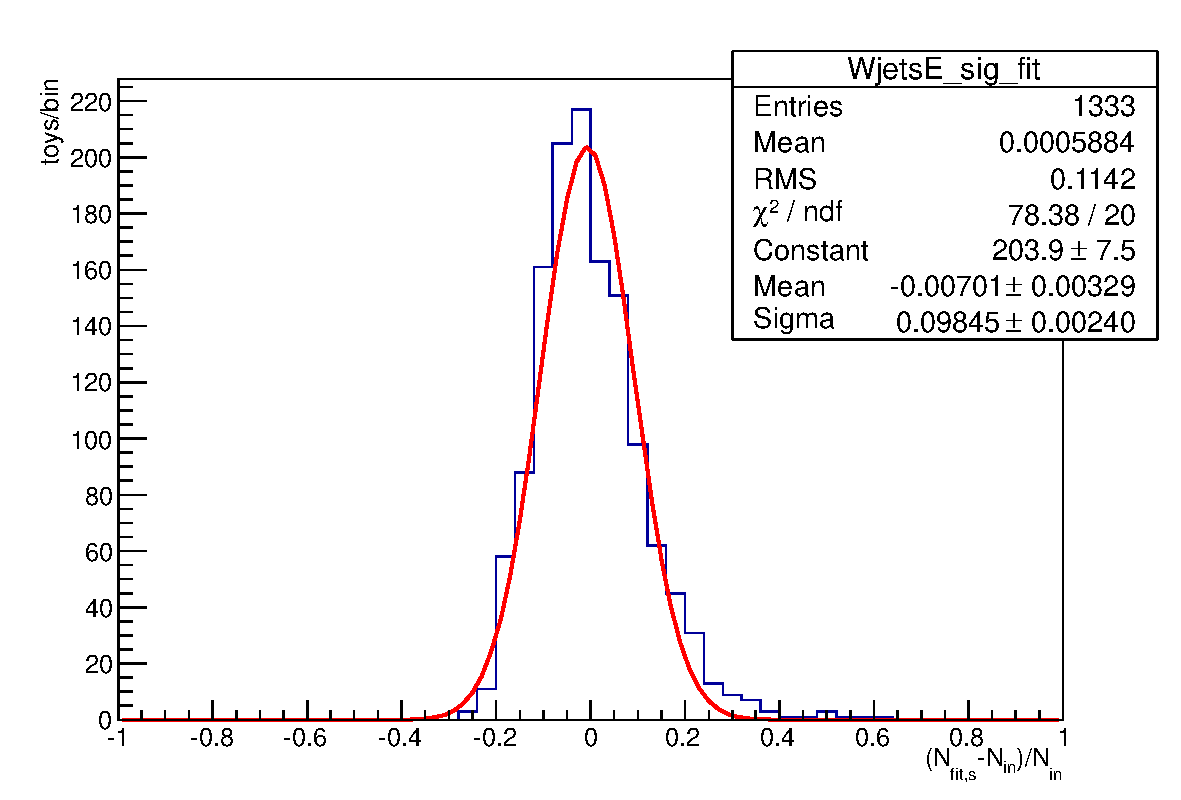
\includegraphics[width=.45\textwidth]{figures/norm_inj125_0j_125_sfit_WjetsE_hww_statonly.pdf}
} 
\subfigure[WjetsM]{
\centering
\label{subfig:wjetsm}
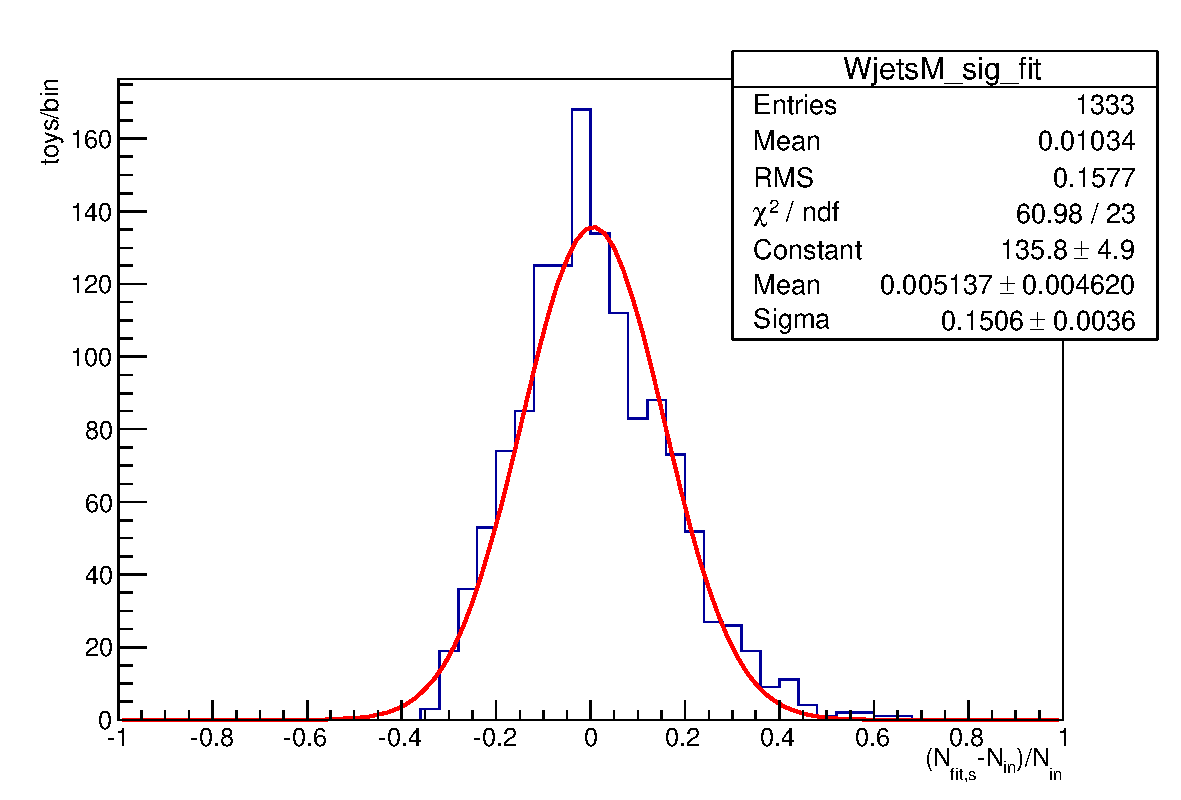
\includegraphics[width=.45\textwidth]{figures/norm_inj125_0j_125_sfit_WjetsM_hww_statonly.pdf}
} 
\subfigure[W$\gamma$]{
\centering
\label{subfig:wgamma}
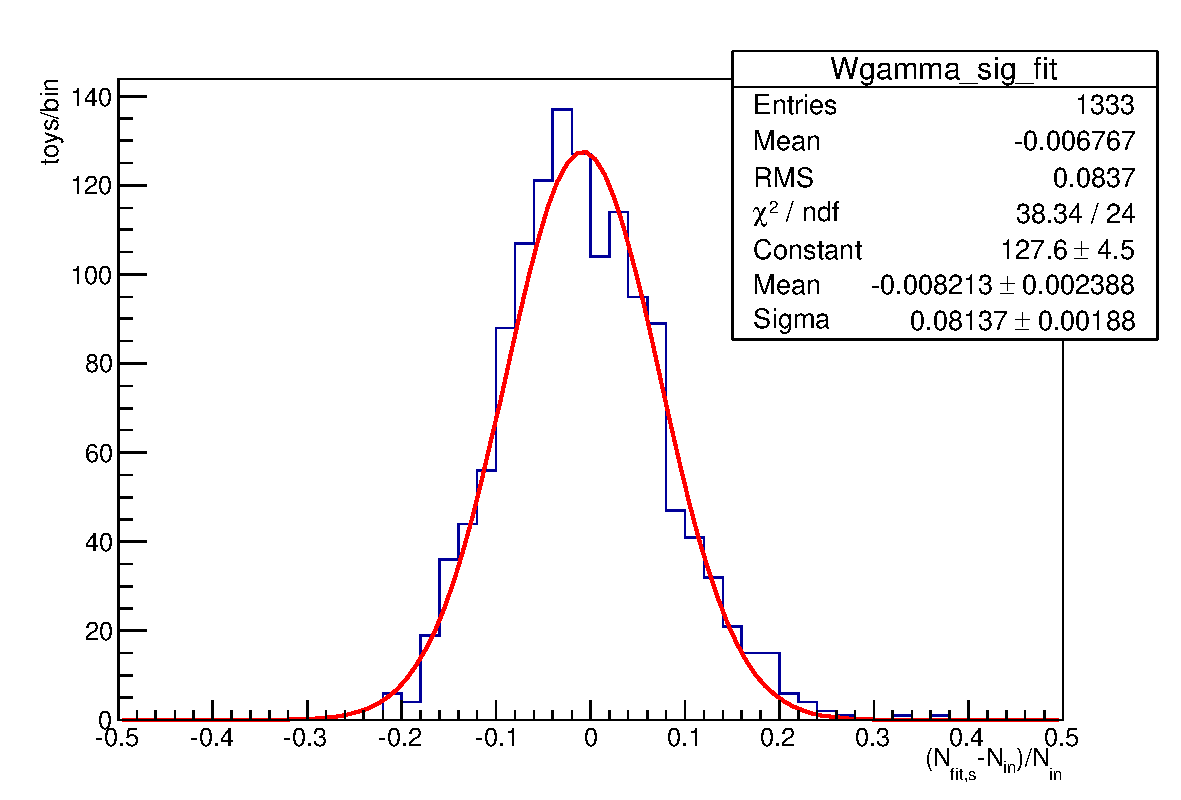
\includegraphics[width=.45\textwidth]{figures/norm_inj125_0j_125_sfit_Wgamma_hww_statonly.pdf}
} 
\subfigure[W$\gamma^*$]{
\centering
\label{subfig:wg3l}
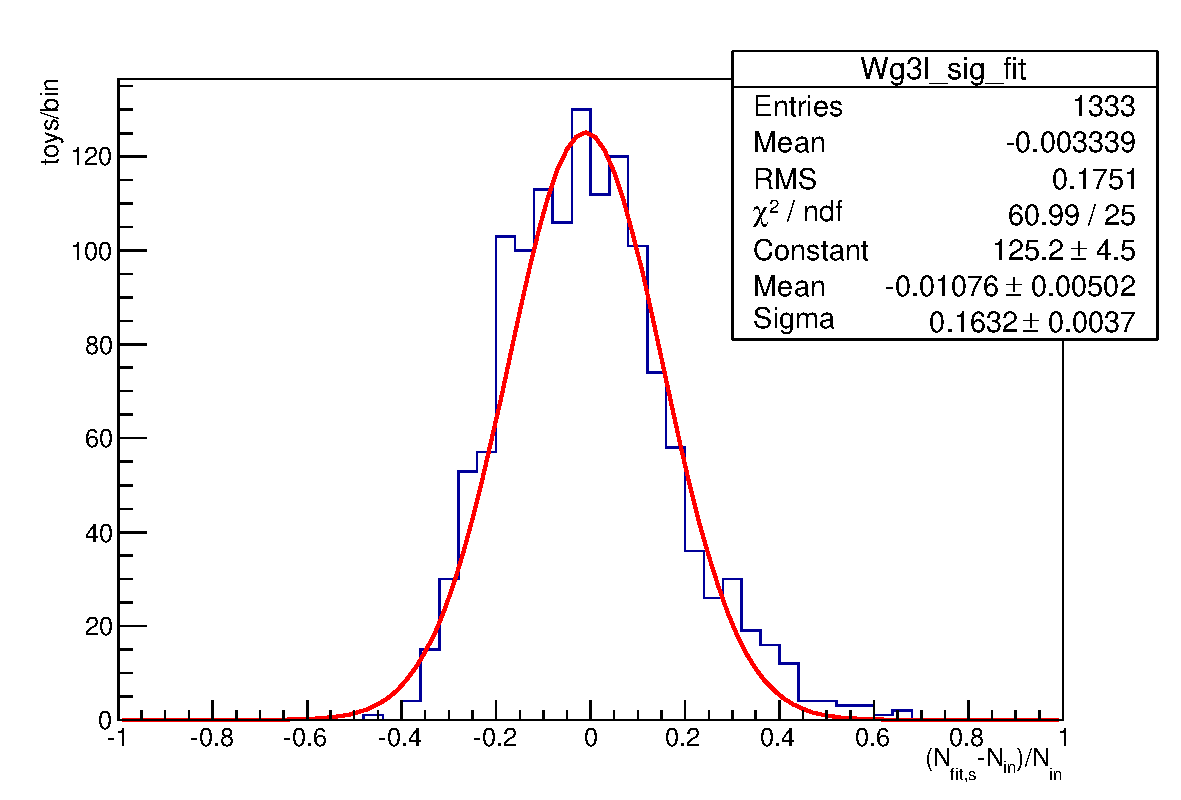
\includegraphics[width=.45\textwidth]{figures/norm_inj125_0j_125_sfit_Wg3l_hww_statonly.pdf}
} 

\caption{The relative fit bias $(N_{\text fit} - N_{\text in})/N_{\text in}$ distributions 
of the main signal and background processes in the toy MC based fit studies in the {\bf 0-Jet bin}. 
The toy datasets are generated sampling {\bf only statistics of the templates}. }
\label{fig:toyfit_statonly_0j}
\end{figure}
%%%%%%%%%%%%%%%%%%%%%%%%%%%%%%%%%%%%


%%%%%%%%%%%%%%%%%%%%%%%%%%%%%%%%%%%%
\begin{figure}[!hbtp]
\centering
\subfigure[ggH]{
\centering
\label{subfig:ggh}
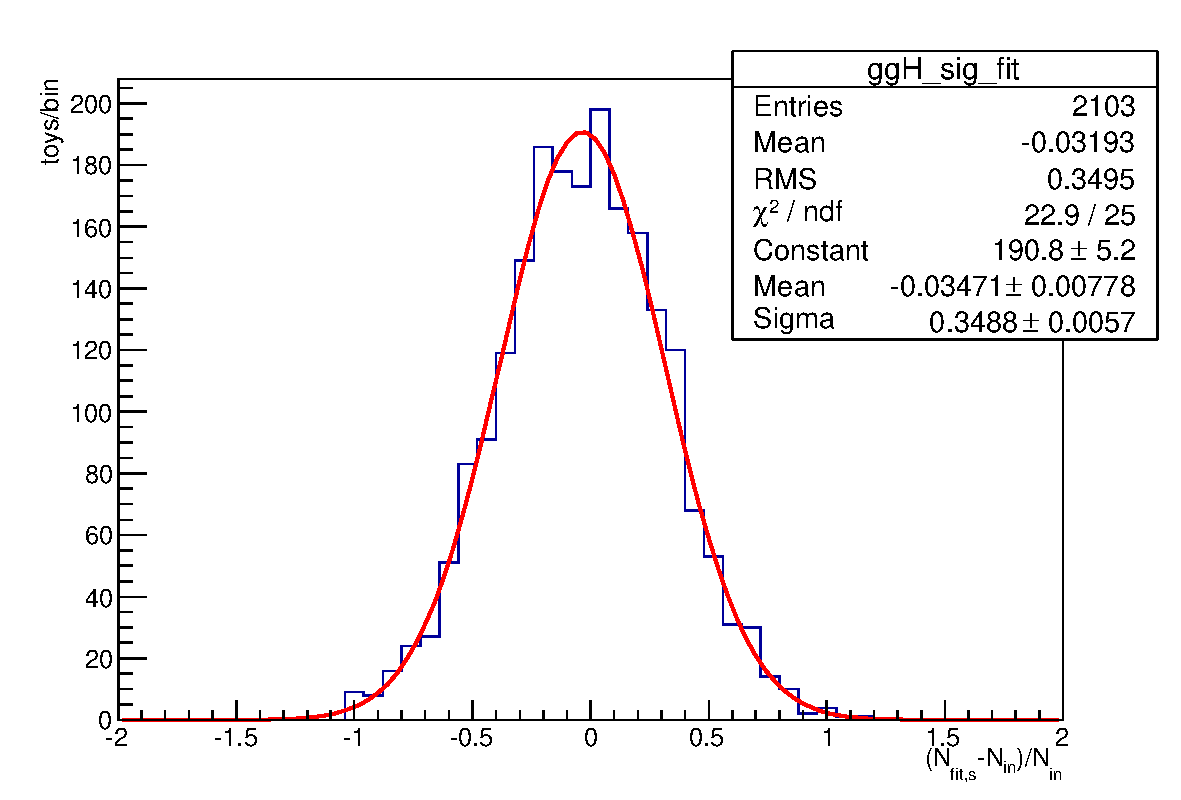
\includegraphics[width=.45\textwidth]{figures/norm_inj125_1j_125_sfit_ggH_hww_statonly.pdf}
}
\subfigure[qqWW]{
\centering
\label{subfig:qqww}
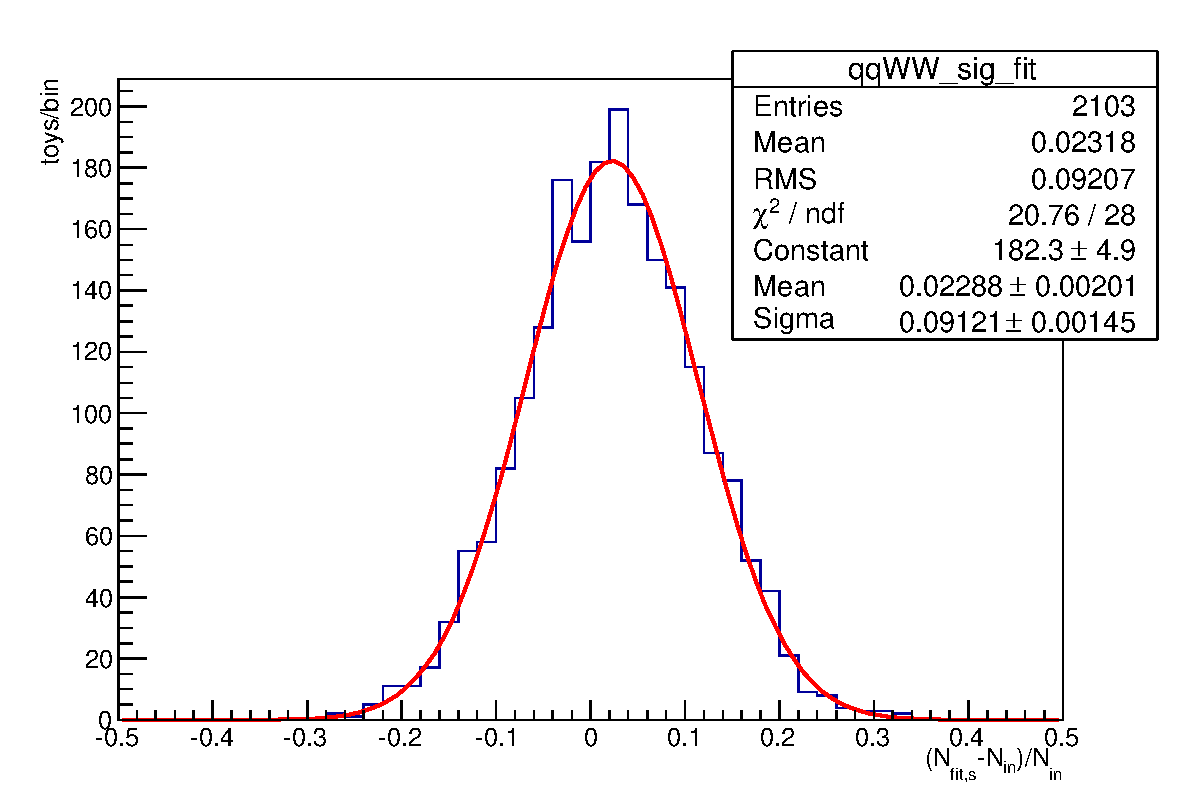
\includegraphics[width=.45\textwidth]{figures/norm_inj125_1j_125_sfit_qqWW_hww_statonly.pdf}
}\\
\subfigure[ggWW]{
\centering
\label{subfig:ggww}
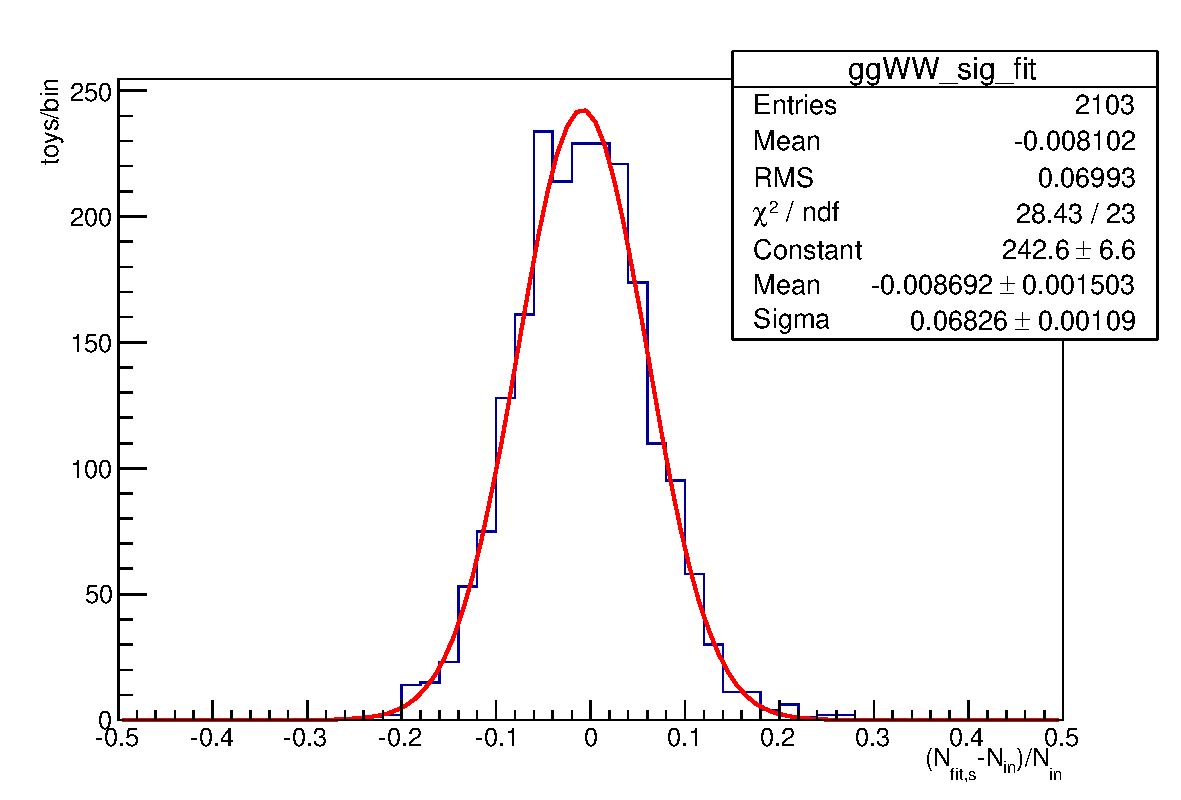
\includegraphics[width=.45\textwidth]{figures/norm_inj125_1j_125_sfit_ggWW_hww_statonly.pdf}
} 
\subfigure[Top]{
\centering
\label{subfig:top}
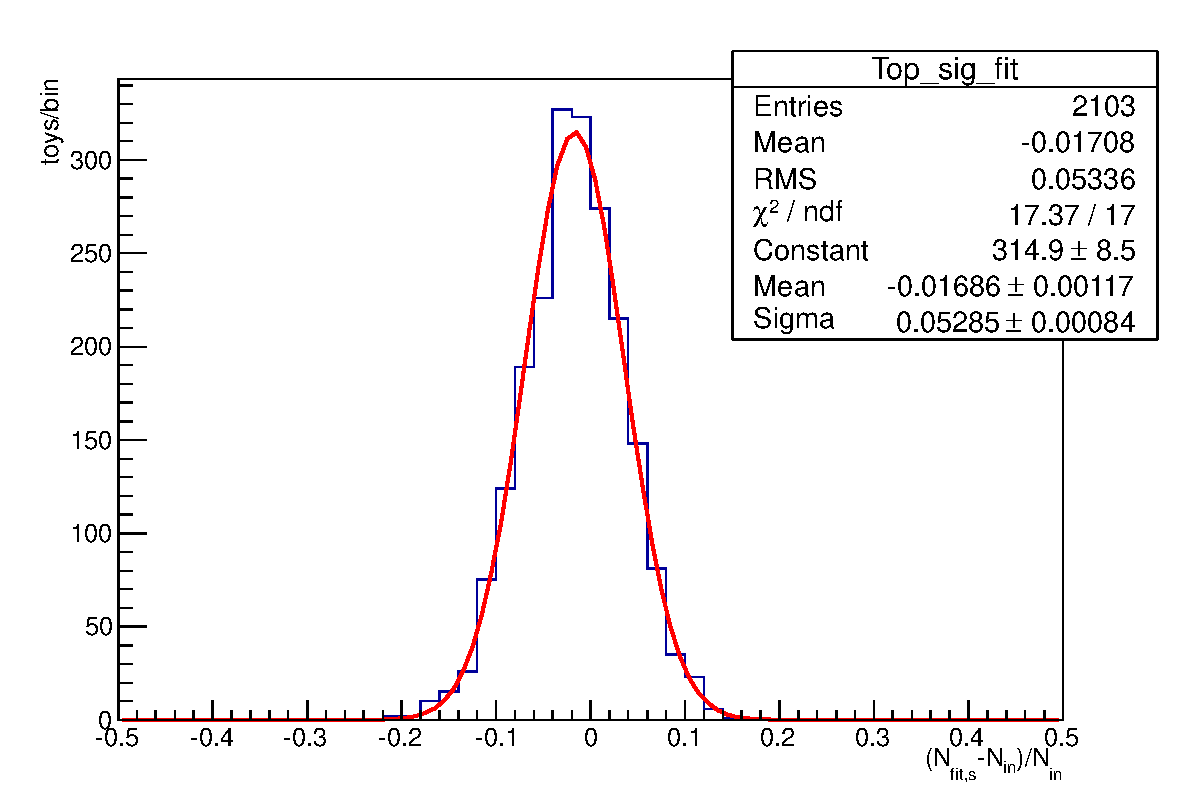
\includegraphics[width=.45\textwidth]{figures/norm_inj125_1j_125_sfit_Top_hww_statonly.pdf}
} \\
\subfigure[WjetsE]{
\centering
\label{subfig:wjetse}
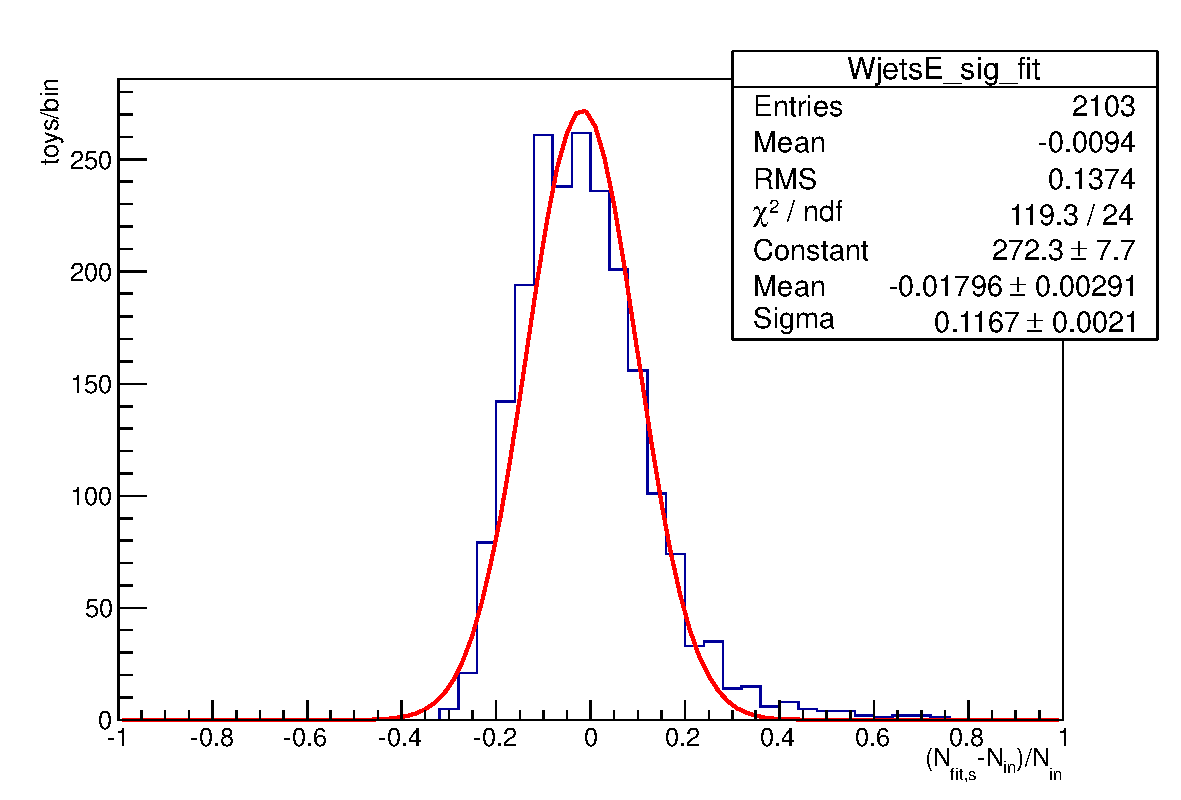
\includegraphics[width=.45\textwidth]{figures/norm_inj125_1j_125_sfit_WjetsE_hww_statonly.pdf}
} 
\subfigure[WjetsM]{
\centering
\label{subfig:wjetsm}
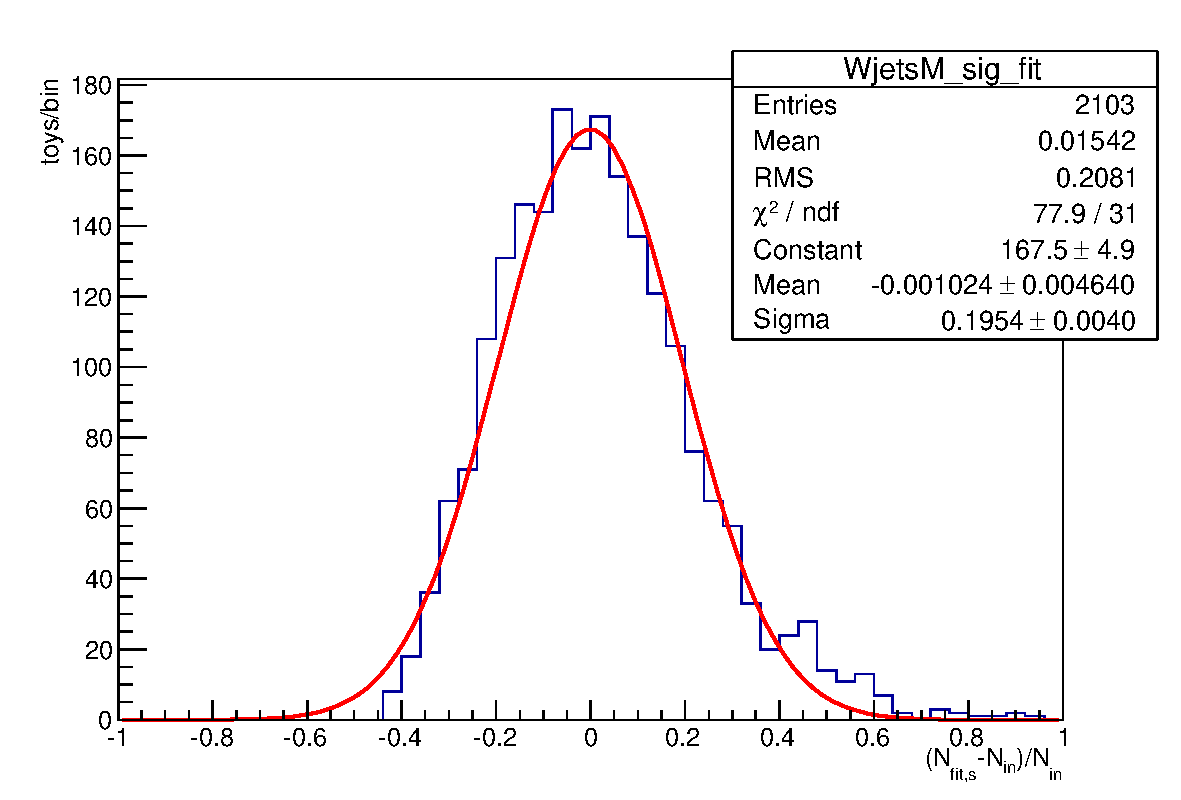
\includegraphics[width=.45\textwidth]{figures/norm_inj125_1j_125_sfit_WjetsM_hww_statonly.pdf}
} 
\subfigure[W$\gamma$]{
\centering
\label{subfig:wgamma}
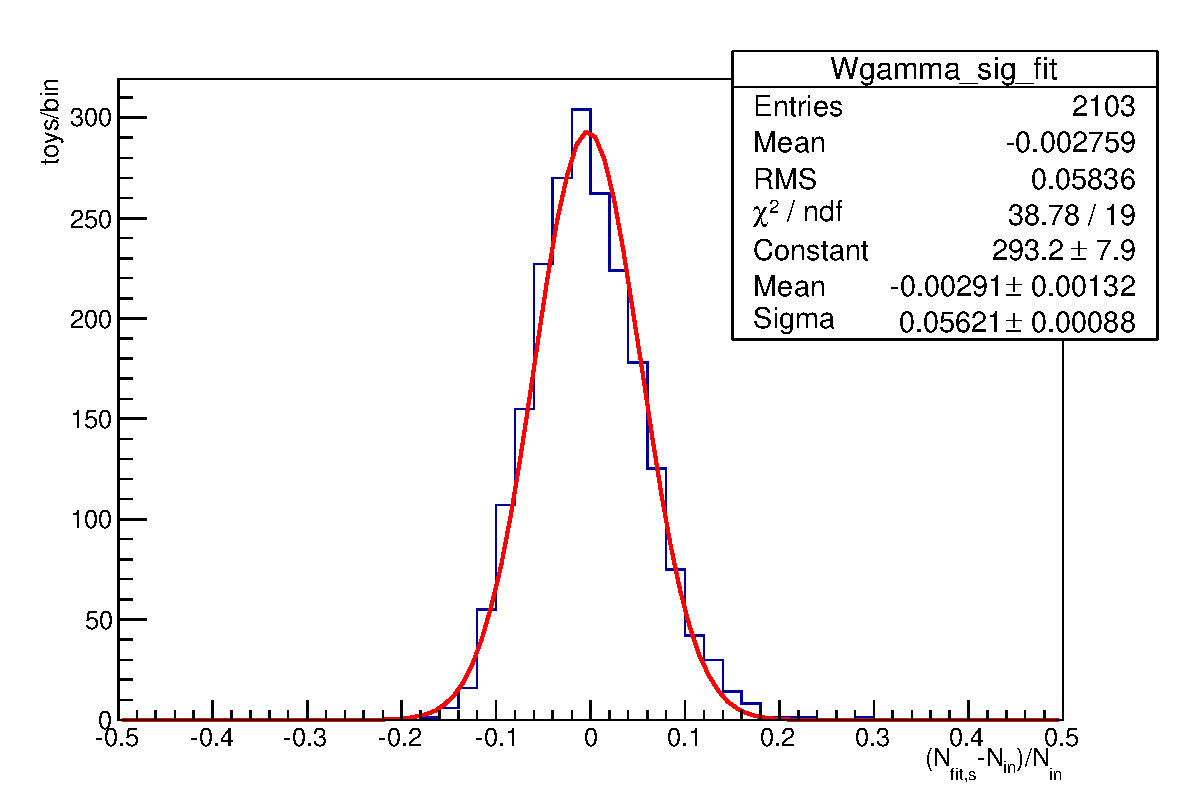
\includegraphics[width=.45\textwidth]{figures/norm_inj125_1j_125_sfit_Wgamma_hww_statonly.pdf}
} 
\subfigure[W$\gamma^*$]{
\centering
\label{subfig:wg3l}
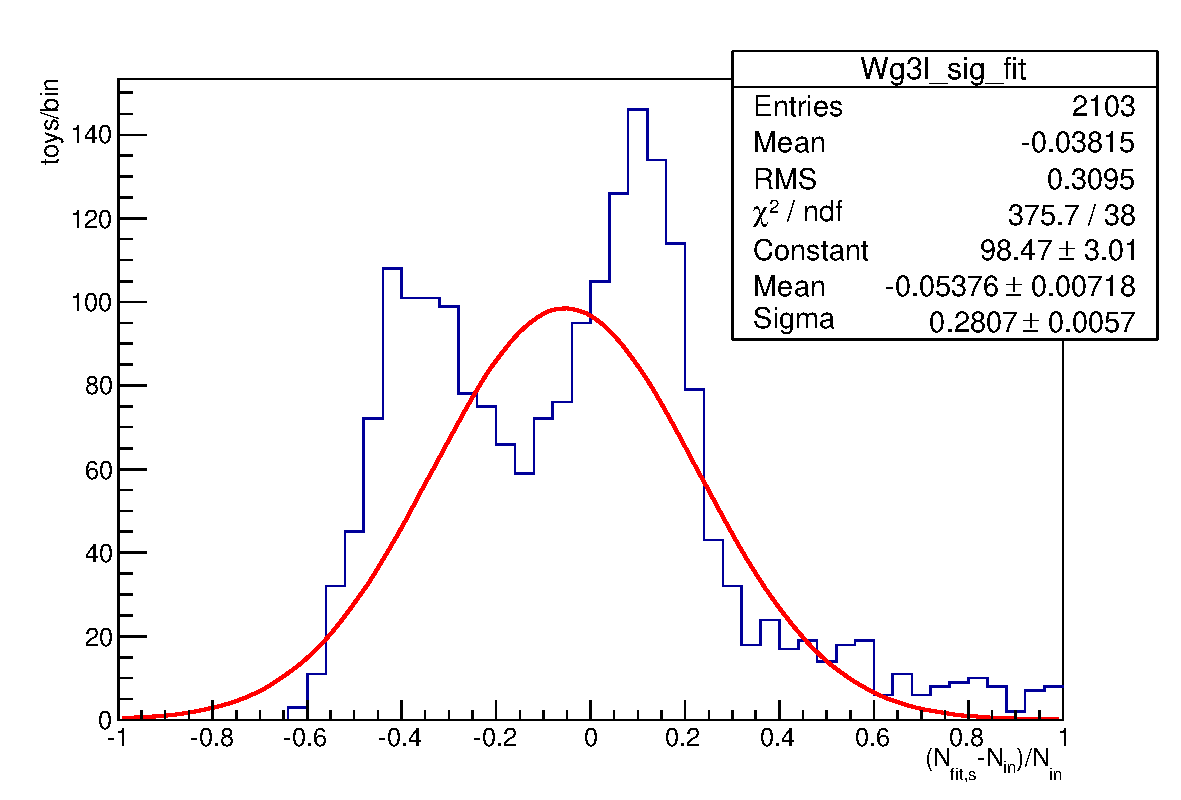
\includegraphics[width=.45\textwidth]{figures/norm_inj125_1j_125_sfit_Wg3l_hww_statonly.pdf}
} 

\caption{The relative fit bias $(N_{\text fit} - N_{\text in})/N_{\text in}$ distributions 
of the main signal and background processes in the toy MC based fit studies in the {\bf 1-Jet bin}. 
The toy datasets are generated sampling {\bf only statistics of the templates}. }
\label{fig:toyfit_statonly_1j}
\end{figure}
%%%%%%%%%%%%%%%%%%%%%%%%%%%%%%%%%%%%


%%%%%%%%%%%%%%%%%%%%%%%%%%%%%%%%%%%%
\begin{figure}[!hbtp]
\centering
\subfigure[ggH]{
\centering
\label{subfig:ggh}
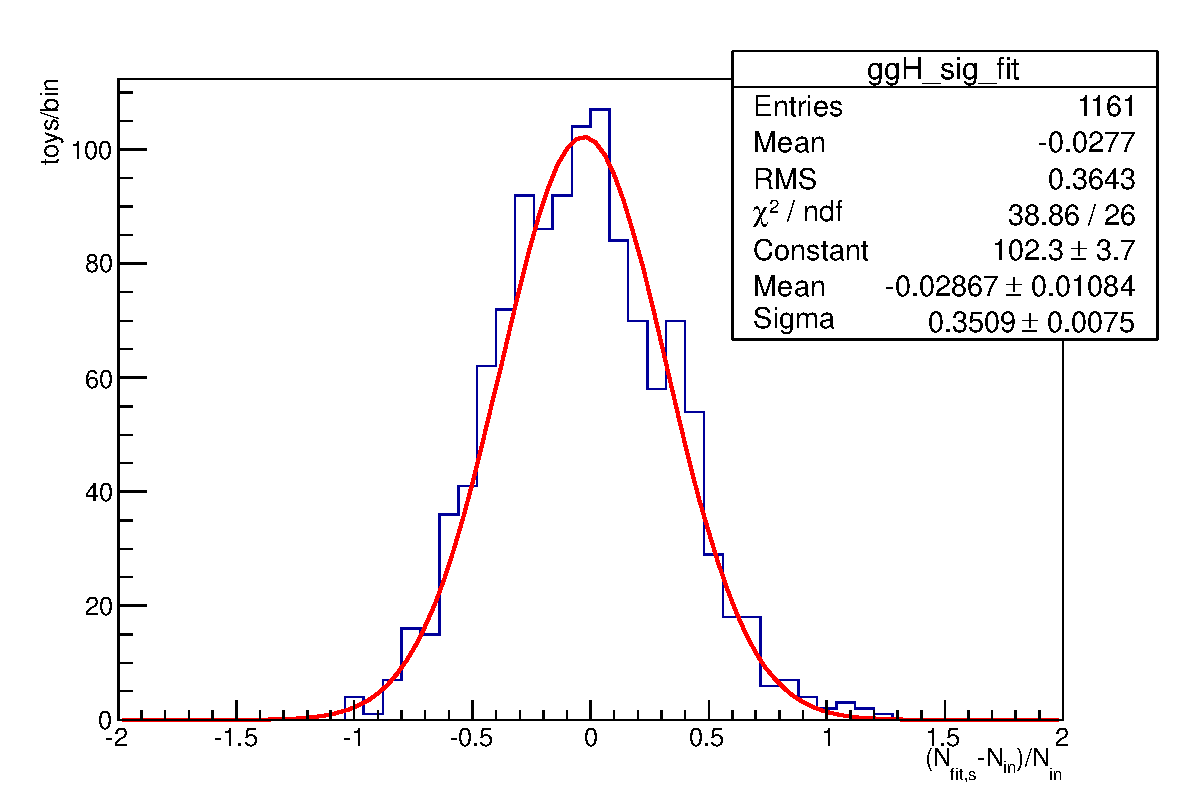
\includegraphics[width=.45\textwidth]{figures/norm_inj125_0j_125_sfit_ggH_hww.pdf}
}
\subfigure[qqWW]{
\centering
\label{subfig:qqww}
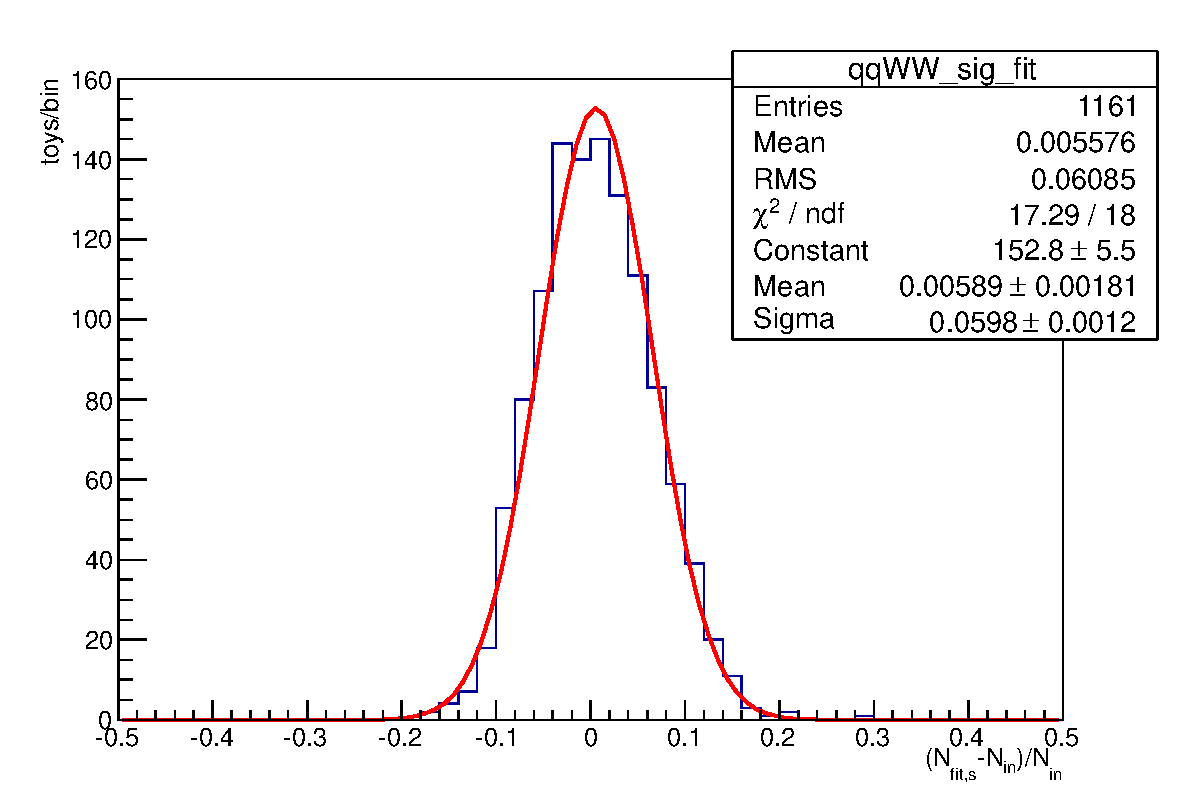
\includegraphics[width=.45\textwidth]{figures/norm_inj125_0j_125_sfit_qqWW_hww.pdf}
}\\
\subfigure[ggWW]{
\centering
\label{subfig:ggww}
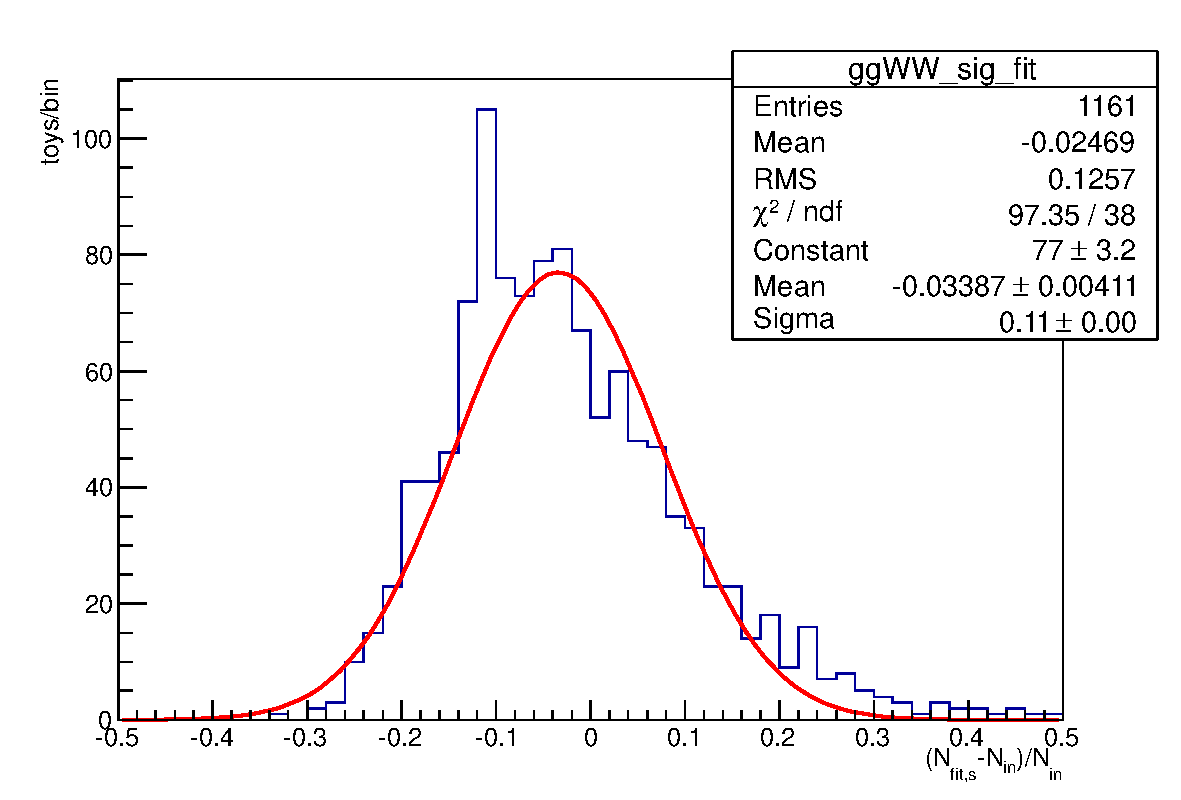
\includegraphics[width=.45\textwidth]{figures/norm_inj125_0j_125_sfit_ggWW_hww.pdf}
} 
\subfigure[Top]{
\centering
\label{subfig:top}
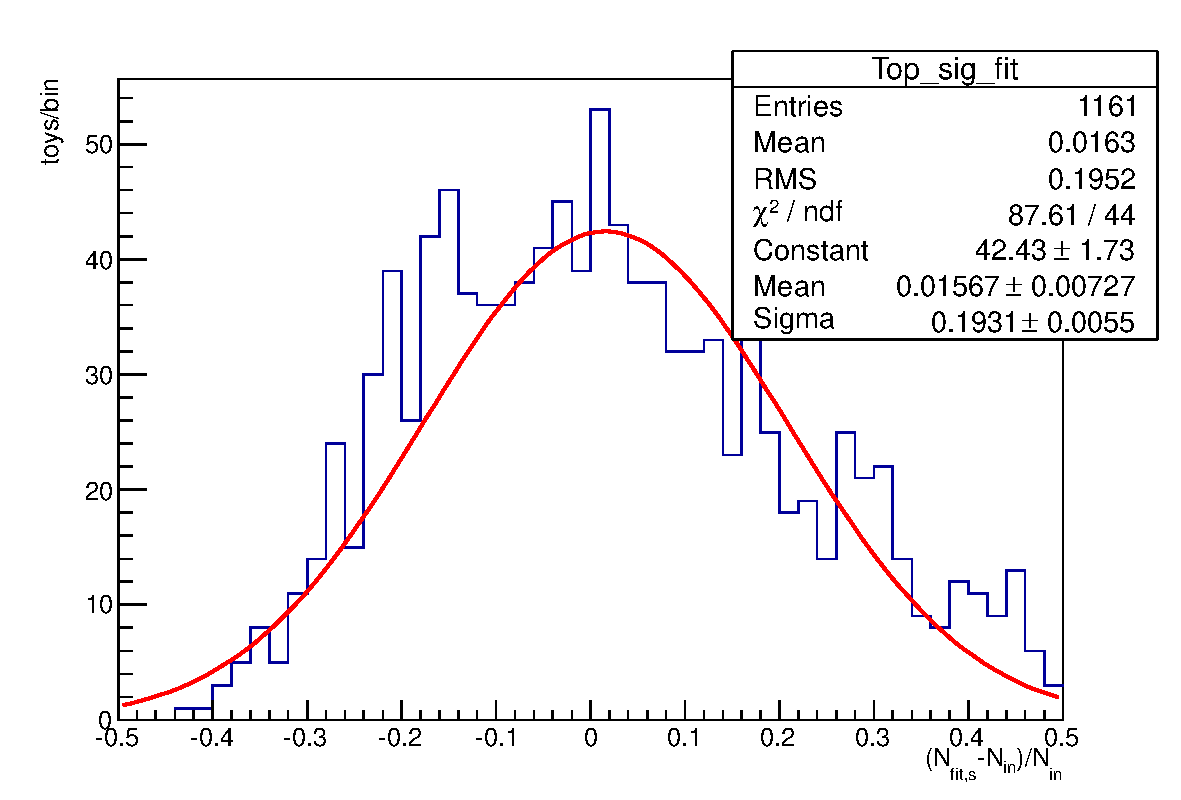
\includegraphics[width=.45\textwidth]{figures/norm_inj125_0j_125_sfit_Top_hww.pdf}
} \\
\subfigure[WjetsE]{
\centering
\label{subfig:wjetse}
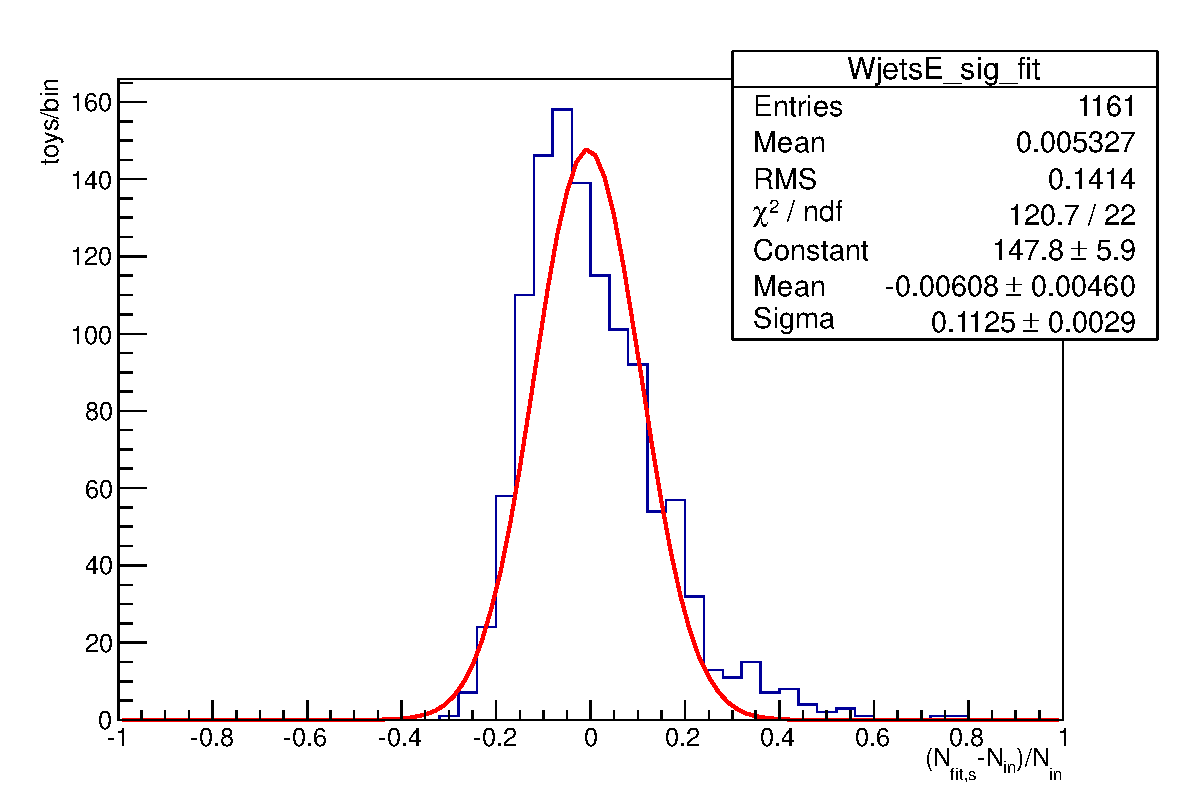
\includegraphics[width=.45\textwidth]{figures/norm_inj125_0j_125_sfit_WjetsE_hww.pdf}
} 
\subfigure[WjetsM]{
\centering
\label{subfig:wjetsm}
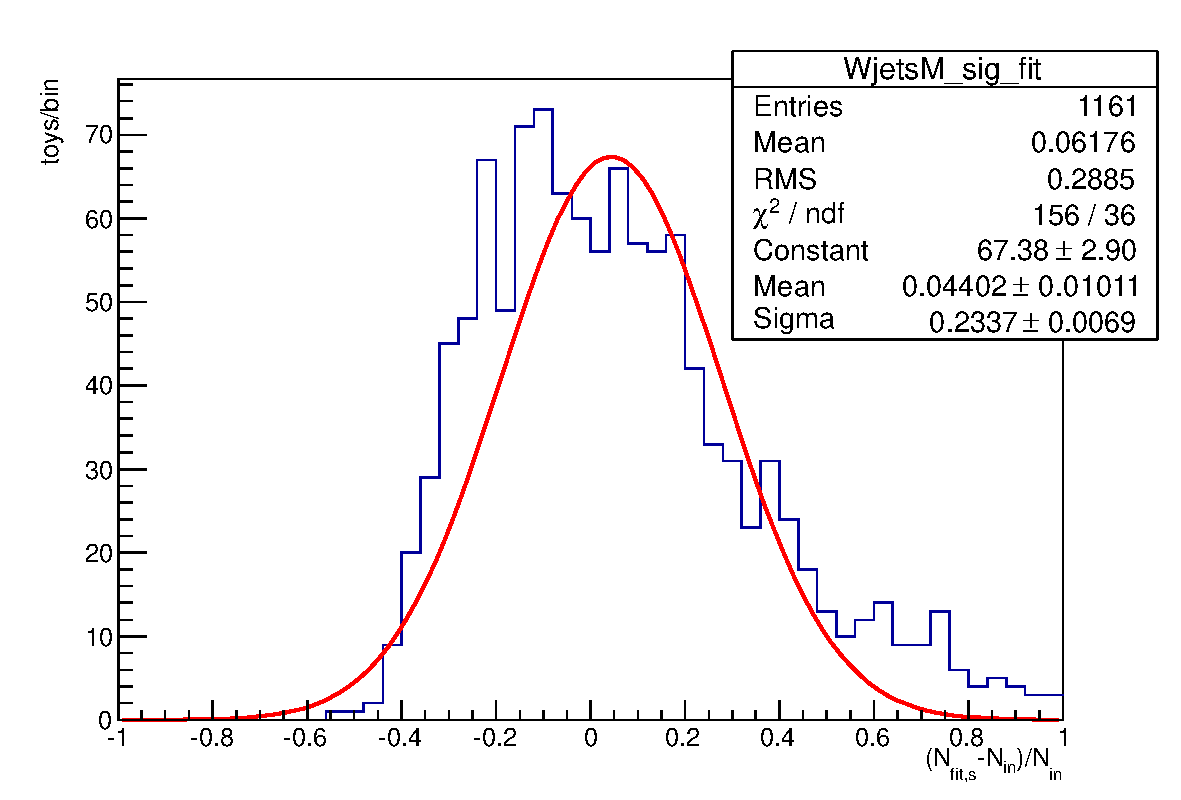
\includegraphics[width=.45\textwidth]{figures/norm_inj125_0j_125_sfit_WjetsM_hww.pdf}
} 
\subfigure[W$\gamma$]{
\centering
\label{subfig:wgamma}
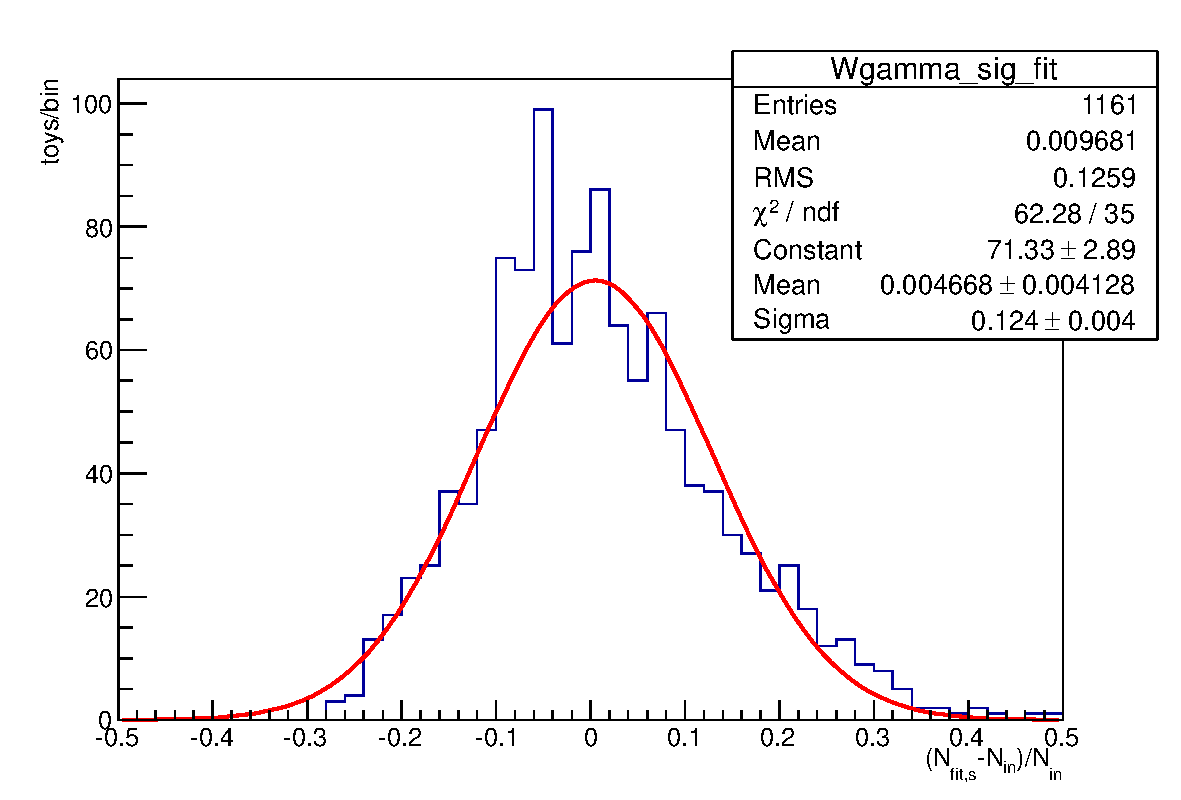
\includegraphics[width=.45\textwidth]{figures/norm_inj125_0j_125_sfit_Wgamma_hww.pdf}
} 
\subfigure[W$\gamma^*$]{
\centering
\label{subfig:wg3l}
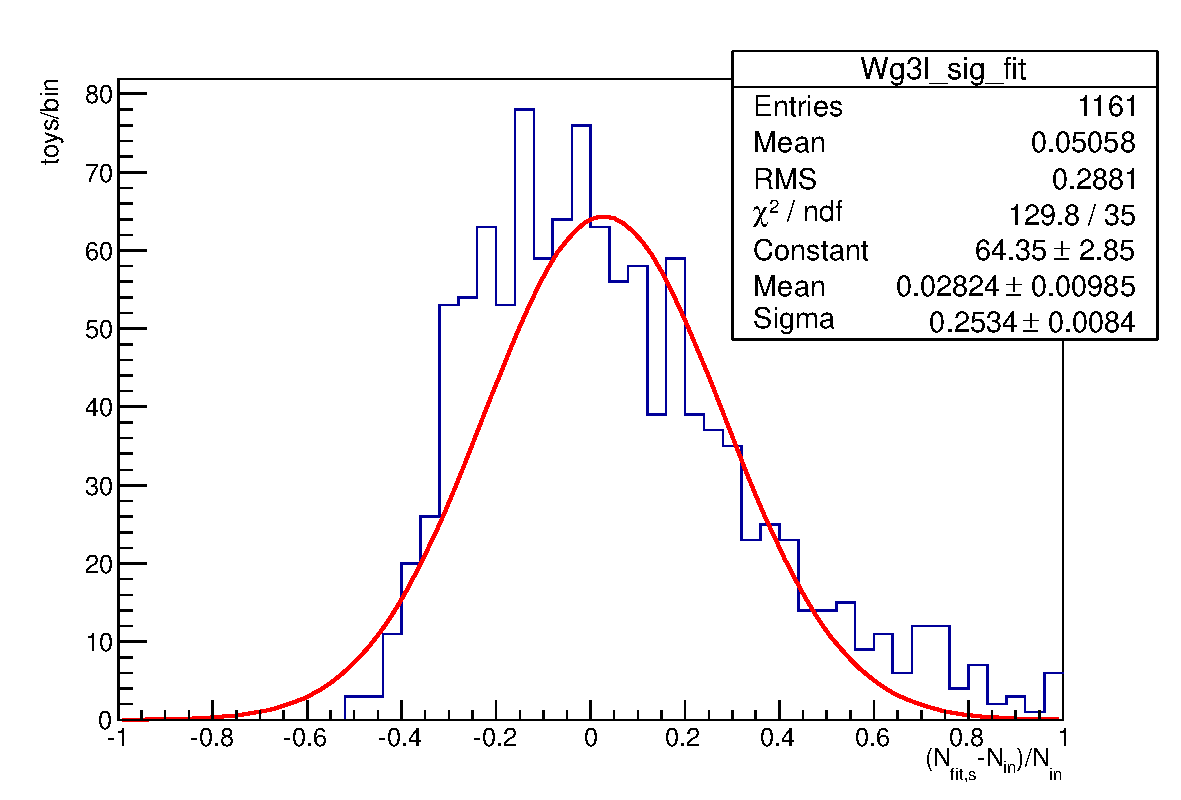
\includegraphics[width=.45\textwidth]{figures/norm_inj125_0j_125_sfit_Wg3l_hww.pdf}
} 

\caption{The relative fit bias $(N_{\text fit} - N_{\text in})/N_{\text in}$ distributions 
of the main signal and background processes in the toy MC based fit studies in the {\bf 0-Jet bin}. 
The toy datasets are generated sampling {\bf both statistics of the templates and systematic nusiances}. }
\label{fig:toyfit_0j}
\end{figure}
%%%%%%%%%%%%%%%%%%%%%%%%%%%%%%%%%%%%


%%%%%%%%%%%%%%%%%%%%%%%%%%%%%%%%%%%%
\begin{figure}[!hbtp]
\centering
\subfigure[ggH]{
\centering
\label{subfig:ggh}
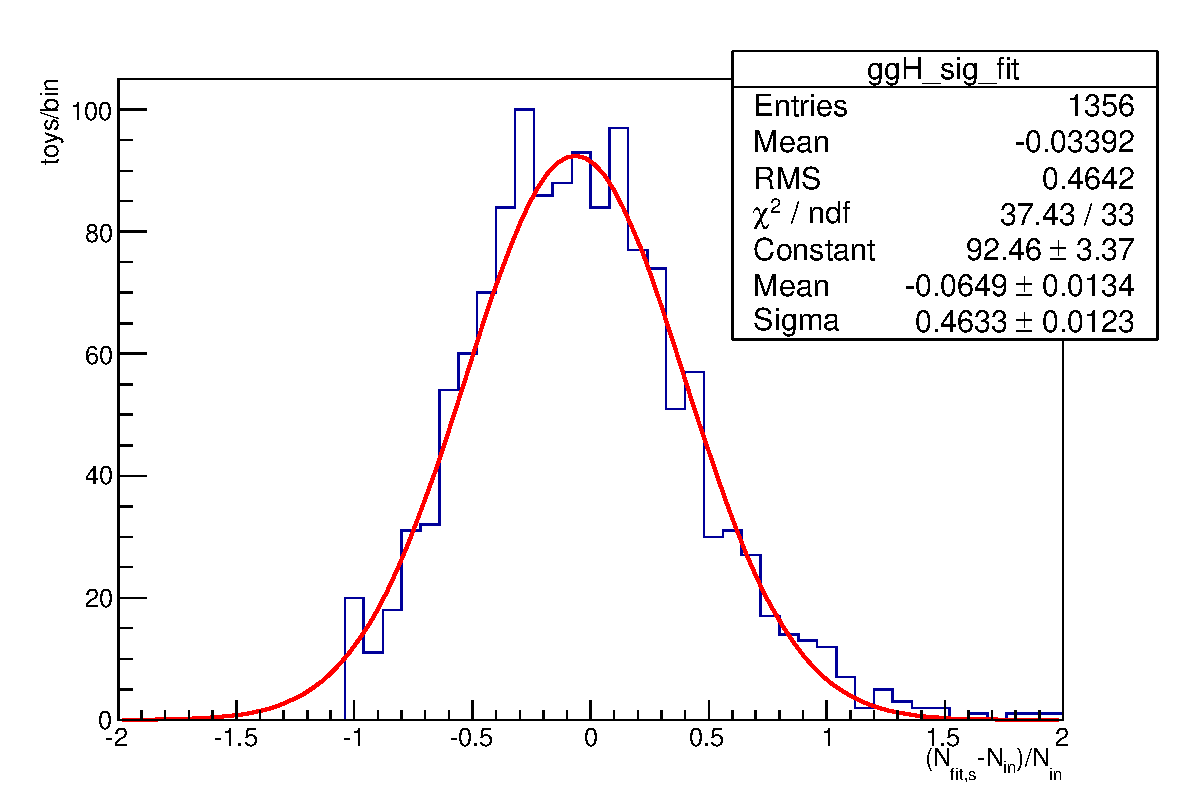
\includegraphics[width=.45\textwidth]{figures/norm_inj125_1j_125_sfit_ggH_hww.pdf}
}
\subfigure[qqWW]{
\centering
\label{subfig:qqww}
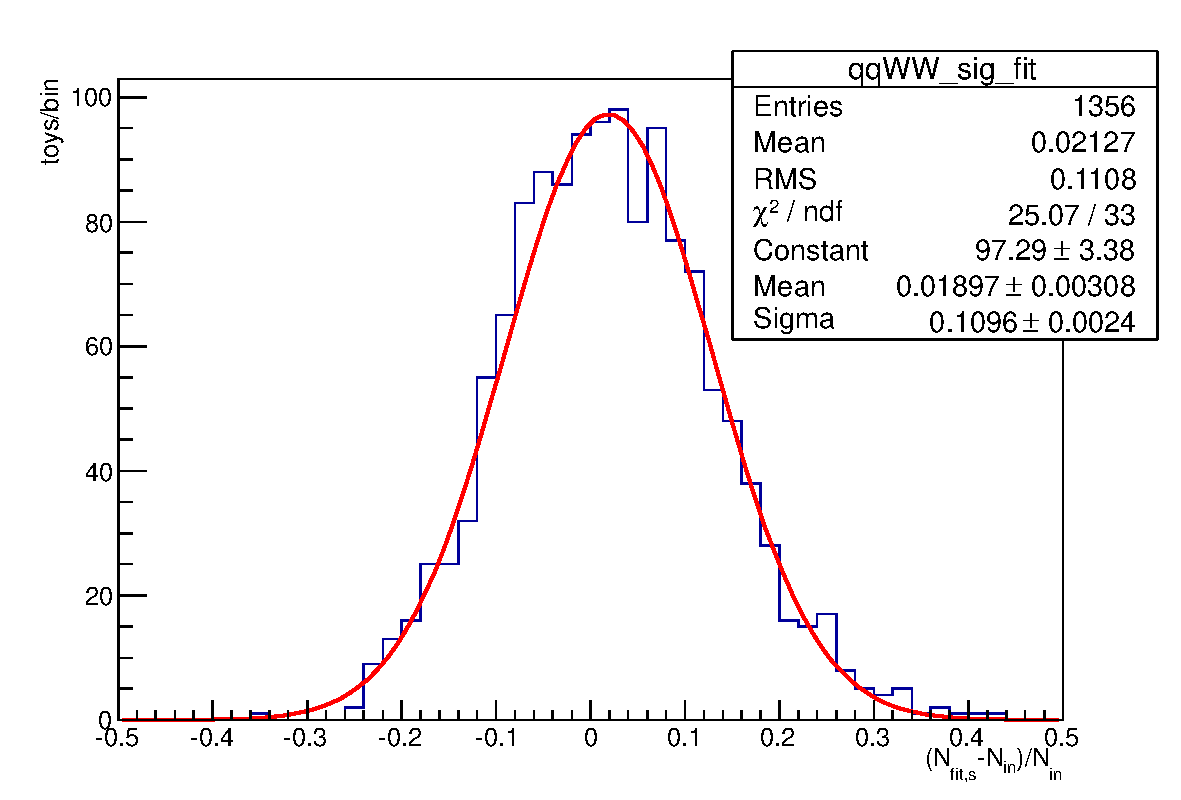
\includegraphics[width=.45\textwidth]{figures/norm_inj125_1j_125_sfit_qqWW_hww.pdf}
}\\
\subfigure[ggWW]{
\centering
\label{subfig:ggww}
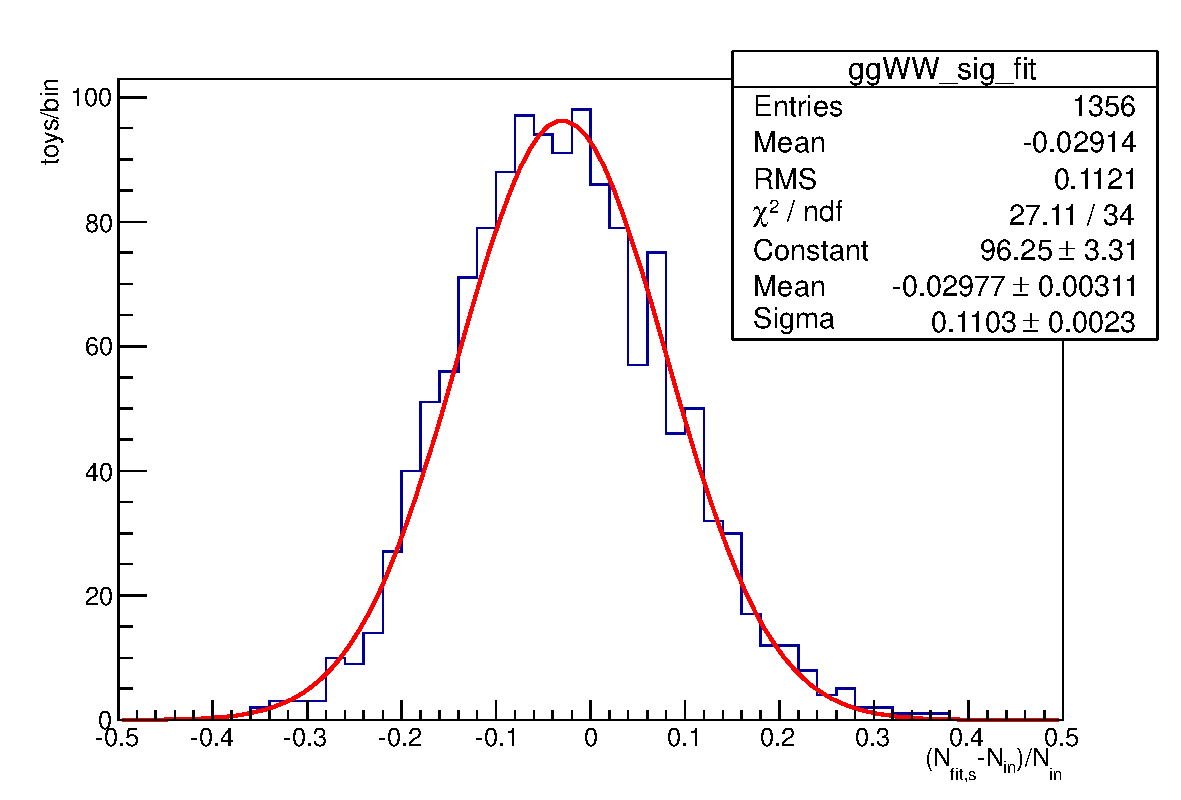
\includegraphics[width=.45\textwidth]{figures/norm_inj125_1j_125_sfit_ggWW_hww.pdf}
} 
\subfigure[Top]{
\centering
\label{subfig:top}
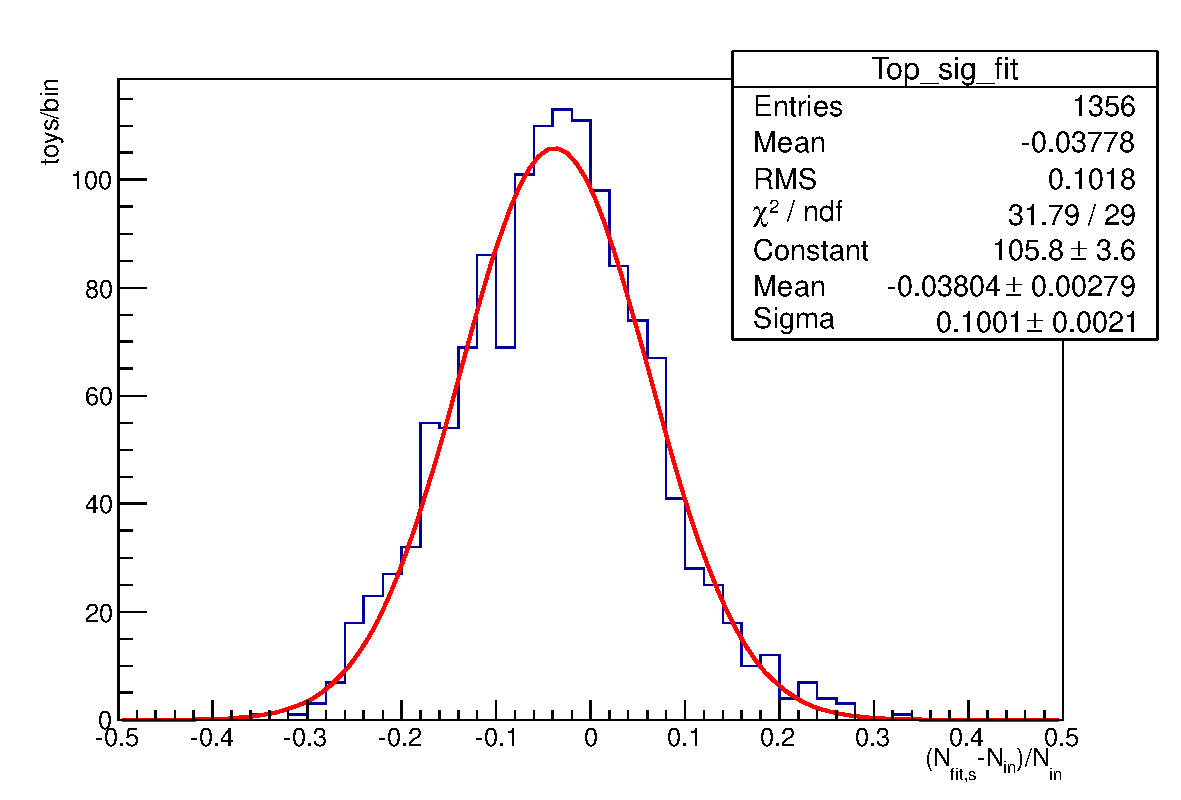
\includegraphics[width=.45\textwidth]{figures/norm_inj125_1j_125_sfit_Top_hww.pdf}
} \\
\subfigure[WjetsE]{
\centering
\label{subfig:wjetse}
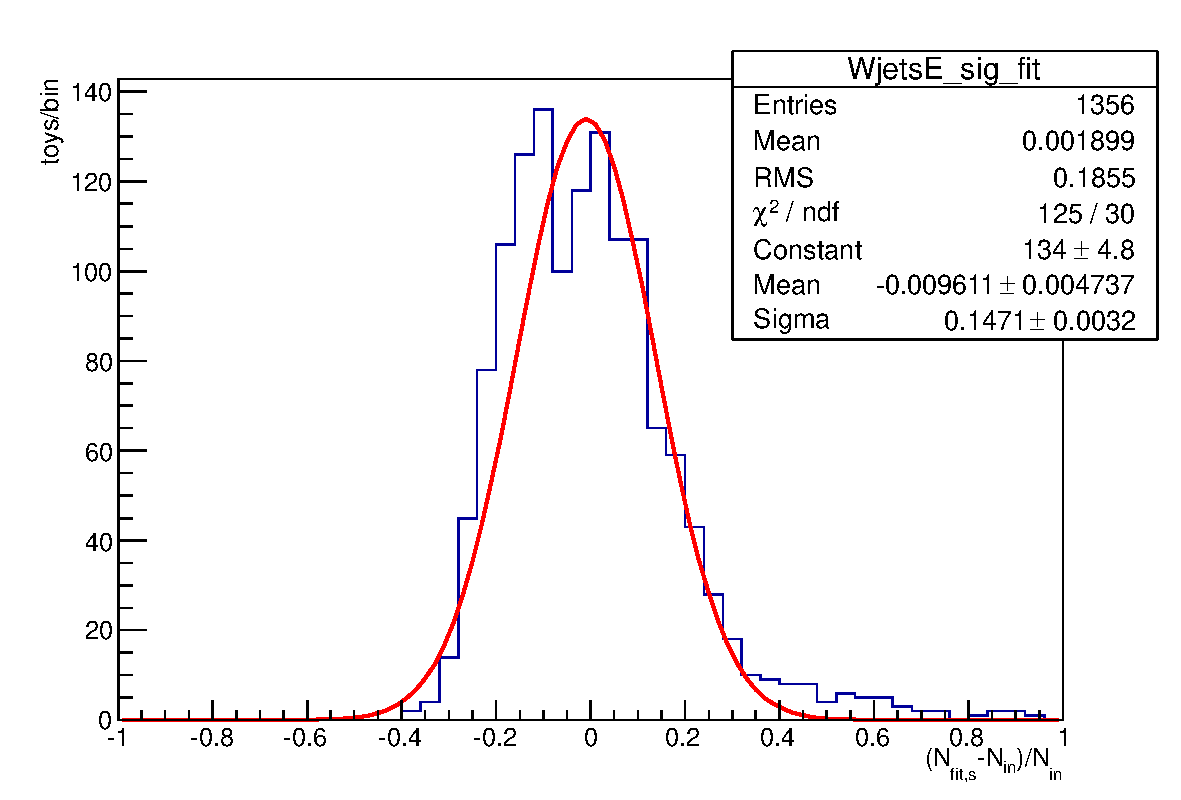
\includegraphics[width=.45\textwidth]{figures/norm_inj125_1j_125_sfit_WjetsE_hww.pdf}
} 
\subfigure[WjetsM]{
\centering
\label{subfig:wjetsm}
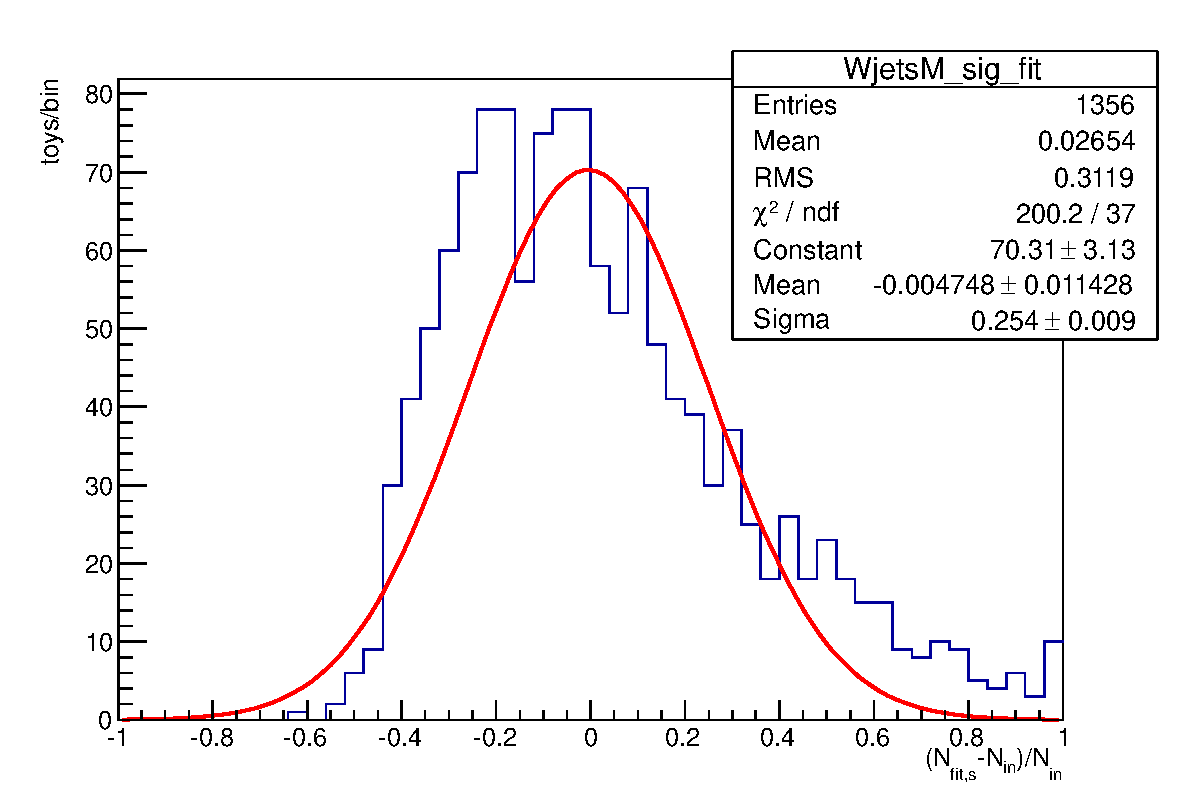
\includegraphics[width=.45\textwidth]{figures/norm_inj125_1j_125_sfit_WjetsM_hww.pdf}
} 
\subfigure[W$\gamma$]{
\centering
\label{subfig:wgamma}
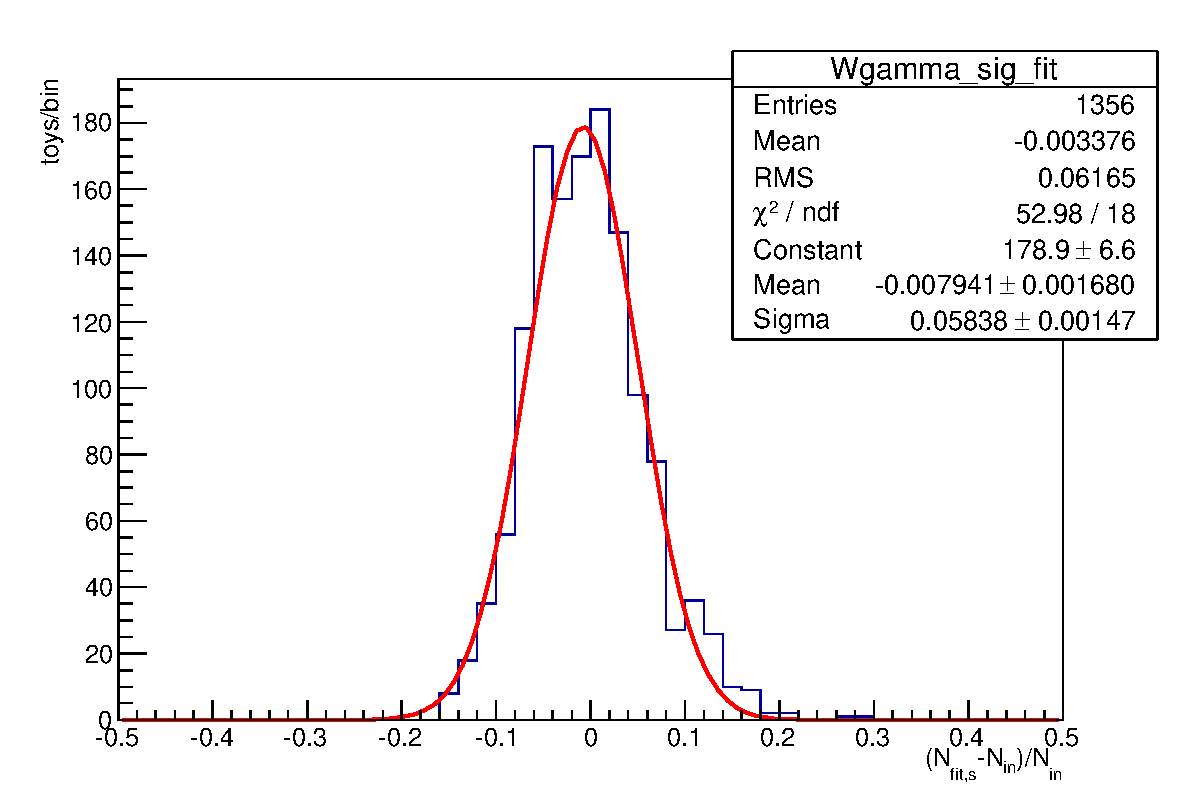
\includegraphics[width=.45\textwidth]{figures/norm_inj125_1j_125_sfit_Wgamma_hww.pdf}
} 
\subfigure[W$\gamma^*$]{
\centering
\label{subfig:wg3l}
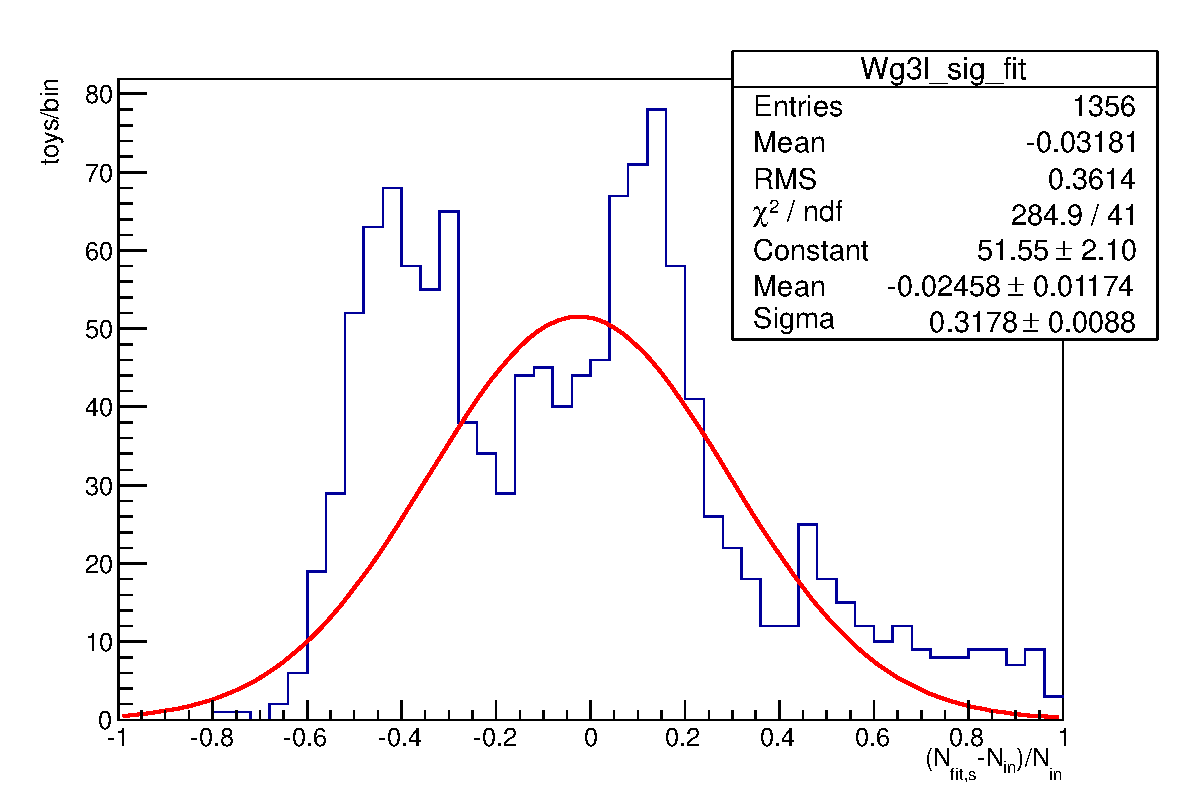
\includegraphics[width=.45\textwidth]{figures/norm_inj125_1j_125_sfit_Wg3l_hww.pdf}
} 

\caption{The relative fit bias $(N_{\text fit} - N_{\text in})/N_{\text in}$ distributions 
of the main signal and background processes in the toy MC based fit studies in the {\bf 1-Jet bin}. 
The toy datasets are generated sampling {\bf both statistics of the templates and systematic nusiances}. }
\label{fig:toyfit_1j}
\end{figure}
%%%%%%%%%%%%%%%%%%%%%%%%%%%%%%%%%%%%




In addition we tested the fit performance in case of problems with the main backgrounds, with the results summarized 
in Table~\ref{tab:toy_summary}.
\begin{itemize}

\item {\bf WjetsM} is a background with about two times as the total signal yield (Table~\ref{tab:yield_summary}) and it has a large normalization uncertainty (36\%). 
Its shape is well constrained but not very different from the signal one. 
Therefore, it is crucial to verify that the fit is stable with respect to WjetsM variations.
First, we tested the ability of the fit to distinguish the signal and WjetsM shapes by relaxing the WjetsM normalization 
without any input bias to the toys: the signal resolution is slightly degraded but no bias is introduced. 
Then, we applied an input bias ($\pm$1$\sigma$ normalization and shape) to the toys and analyzed them with the nominal analysis. 
The normalization bias is a large effect and the fit is only partially able to absorb it into the WjetsM component; 
the resulting bias on the signal is about 6\% (resolution is unaffected). 
The largest bias on the signal yield is 14\%, from the 1-Jet where the WjetsM background input is -36\% less than what 
the nominal fit assume.

\item {\bf qqWW} is the largest background; it is well constrained both in terms of normalization and shape, but small variations of this 
process have a large size with respect to the signal. 
We tested variations on normalization ($\pm$10\%, roughly equal to 1$\sigma$ in the 0-jet bin), 
on shape (using the alernative shape from MCatNLO as input to the toys) and on both. 
In all cases, the effect on the signal is small, with biases $\leq$1\% in the 0-Jet.  
%As expected, when relaxing the qqWW normalization uncertainty, it is easier for the fit to account the observed bias to the qqWW process,
%and consequently reduce the already small signal bias (by a factor of 2).

\item {\bf Top} is the main background in the 1-jet bin. 
We tested variations on normalization - $\pm$20\% (5\%), roughly equal to 1$\sigma$ in the 0-jet (1-jet) bin - and on shape 
(using the alernative shape from MadGraph as input to the toys) separately. No bias is introduced for the signal. 
It is interesting to note that, in case of normalization bias in the 1-jet bin, the fit prefers to account the observed bias 
into the qqWW component since it has similar shape but larger normalization error. However even in that case the impact 
on the signal yield is low being 6\%. 
\end{itemize}

In summary, we find the fit to be very stable with respect to biases at the level of 1$\sigma$ both in terms of shape and 
normalization for the main backgrounds. The largest observed bias is 14\% when injecting a 36\% less Wjets than expected 
in the 1-jet bin.
We also repeated the studies on the HCP analysis with results given in Appendix~\ref{sec:appendix_fittoyshcp}. 

%%%%%%%%%%%%%%%%%%%%%%%%%%%%%% 
\begin{table}
\begin{center}
\begin{tabular}{c | c  | c c | c c | c c | c c | c c }
\hline
          &      & \multicolumn{2}{c|}{{\bf ggH}} & \multicolumn{2}{c|}{qqWW} & \multicolumn{2}{c|}{Top} & \multicolumn{2}{c}{WjetsM} & \multicolumn{2}{c}{WjetsE} \\ 
N$_{jets}$ & Test & bias & $\sigma$ & bias & $\sigma$ & bias & $\sigma$ & bias & $\sigma$ & bias & $\sigma$ \\
\hline
0 & default                             &  2  & 28 & 0.4 & 3 & 0.4 & 11 & 0.5 & 15 & 0.7 & 10 \\
0 & sampling: stat.+syst.               &  4  & 36 & 0.6 & 7 &  3  & 21 &  6  & 25 & 0.2 & 11 \\
\hline
0 & analysis: inflated Wjets error      &  2  & 29 & -0.3 & 3 & 0.2 & 12 & -0.2      & 19 & -0.6 & 10 \\
0 & input: WjetsM {\bf +36\% bias}      &  6  & 28 & 0.3  & 3 & 0.8 & 11 & {\bf 27}  & 18 & 4    & 10 \\
0 & input: WjetsM {\bf -36\% bias}      & -6  & 25 & -1   & 3 & 3   & 11 & {\bf -23} & 10 & -7   & 10 \\
0 & input: WjetsM from altern. shape    & -4  & 25 & -0.1 & 3 & 2   & 11 & 6         & 15 & -0.5 & 10 \\
\hline
0 & input: qqWW {\bf +10\% bias}        & 0.7 & 28 & {\bf 10}  & 3 & 0.8 & 12 & 0.5 & 14 & 0.4 & 10 \\
0 & input: qqWW {\bf -10\% bias}        & 0.2 & 26 & {\bf -10} & 3 & 0.1 & 11 & 0.4 & 15 & 0.4 & 10 \\
0 & input: qqWW from altern. shape      & -2  & 27 & -0.1      & 3 & 2   & 12 & 6   & 15 & -2  & 10 \\
\hline
0 & input: Top {\bf +20\% bias}         & -2  & 27  & 1    & 3 & {\bf 11} & 12  & -0.5 & 15  & -1   & 9\\
0 & input: Top {\bf -20\% bias}         & 3   & 27  & -2   & 3 & {\bf -9} & 10  & 2    & 16  & -0.8 & 10\\
0 & input: Top from altern. shape       & -2  & 27  & -0.6 & 3 & 5        & 11  & 8    & 16  & -1   & 9\\
\hline
\hline
1 & default                             & -3  & 35 & 2   & 9  & -2  & 5 & -0.1 & 20 & -2 & 12 \\
1 & sampling: stat.+syst.               & -6  & 48 & 3   & 16 & 0.4 & 6 & 0.6  & 25 & 0.7& 14 \\
\hline
1 & analysis: inflated Wjets error      &  -3 &  37 & 2  & 9 & -2   & 5  & 0.1      & 24  & -2  & 12 \\ 
1 & input: WjetsM {\bf +36\% bias}      &  5  &  35 & 4  & 9 & -2   & 5  & {\bf 26} & 26  & 1   & 12 \\ 
1 & input: WjetsM {\bf -36\% bias}      & -14 &  33 & 0.5& 9 & -1   & 5  & {\bf-20} & 15  & -5  & 11 \\ 
1 & input: WjetsM from altern. shape    &  -3 &  35 & 1  & 8 & -0.3 & 5  & 17       & 21  & -1  & 12 \\
\hline
1 & input: qqWW {\bf +10\% bias}        & 4   & 37 & {\bf 12} & 9 & -2  & 5  & 0.3  & 19 & 1  & 11 \\
1 & input: qqWW {\bf -10\% bias}        & -1  & 33 & {\bf -7} & 9 & -2  & 5  & 0.3  & 18 & -2 & 13 \\
1 & input: qqWW from altern. shape      & -2  & 37 & 2        & 8 & -1  & 4  & 14   & 22 & -3 & 12 \\
\hline
1 & input: Top {\bf +5\% bias}          & -6   & 35  & 8   & 9 & {\bf -0.5} & 5 & -1 & 17 & -2 & 11 \\
1 & input: Top {\bf -5\% bias}          & -2   & 35  & -2  & 9 & {\bf -3}   & 5 & 2  & 19 & -1 & 12 \\
1 & input: Top from altern. shape       & -0.3 & 33  & 0.6 & 8 & 0.3        & 5 & 17 & 21 & -2 & 12 \\
\hline
\hline
\end{tabular}
\caption{Summary of results from toy experiments. Values of bias and $\sigma$ are \%.
In the Test column, ``default'' stands for: sampling is statistical only, input is nominal, analysis is nominal; 
in all other cases, the difference with respect to default is stated.}
\label{tab:toy_summary}
\end{center}
\end{table}


%%%%%%%%%%%%%%%%%%%%%%%%%%%%%% 
\begin{table}
\begin{center}
\begin{tabular}{c | c c c c c | c  c  c c c }
\hline
N$_{jets}$ & ggH & qqWW & Top & WjetsM & WjetsE & ggH/qqWW & ggH/Top & ggH/WjetsM & ggH/WjetsE \\
\hline
0 & 237.4 & 3930.1 & 488.9  & 512.4 & 276.4 & 6\% & 49\% & 46\% &  86\%\\
1 & 91.2  & 1177.5 & 1429.4 & 226.9 & 128.0 & 8\% & 64\% & 40\% &  71\%\\
\hline
\end{tabular}
\caption{Summary of yields and relative fraction of the signal with respect to the main backgrounds.}
\label{tab:yield_summary}
\end{center}
\end{table}

